\documentclass[conference]{IEEEtran}
\IEEEoverridecommandlockouts
% The preceding line is only needed to identify funding in the first footnote. If that is unneeded, please comment it out.
\usepackage{cite}
\usepackage{amsmath,amssymb,amsfonts}
\usepackage{algorithmic}
\usepackage{graphicx}
\usepackage{multirow}
\usepackage{booktabs}
\usepackage{textcomp}
\usepackage{hyperref}
\usepackage{xcolor}
\def\BibTeX{{\rm B\kern-.05em{\sc i\kern-.025em b}\kern-.08em
    T\kern-.1667em\lower.7ex\hbox{E}\kern-.125emX}}
\begin{document}

\title{Decipherable Classification of Glaucoma using
Deep Neural Network Leveraging XAI\\
}

\author{\IEEEauthorblockN{Touhidul Islam Chayan}
\IEEEauthorblockA{\textit{Department of Computer Science and Engineering} \\
\textit{BRAC University}\\
Dhaka, Bangladesh \\
touhidul.islam.chayan@g.bracu.ac.bd}
\and
\IEEEauthorblockN{Anita Islam}
\IEEEauthorblockA{\textit{Department of Computer Science and Engineering} \\
\textit{BRAC University}\\
Dhaka, Bangladesh \\
anita.islam@g.bracu.ac.bd}
\and
\IEEEauthorblockN{Tonny Anika Rahman}
\IEEEauthorblockA{\textit{Department of Computer Science and Engineering} \\
\textit{BRAC University }\\
Dhaka, Bangladesh \\
anika.rahman.tonny@g.bracu.ac.bd}
\and
\IEEEauthorblockN{Eftykhar Rahman}
\IEEEauthorblockA{\textit{Department of Computer Science and Engineering} \\
\textit{BRAC University}\\
Dhaka, Bangladesh \\
eftykhar.rahman@g.bracu.ac.bd}

\and
\IEEEauthorblockN{Md. Tanzim Reza}
\IEEEauthorblockA{\textit{Department of Computer Science and Engineering} \\
\textit{BRAC University}\\
Dhaka, Bangladesh \\
tanzim.reza@bracu.ac.bd}
\and
\IEEEauthorblockN{Mohammad Zavid Parvez}
\IEEEauthorblockA{\textit{Lecturer} \\
\textit{Engineering Institute of Technology}\\
Australia\\
zavid.parvez@bracu.ac.bd}
}

\maketitle

\begin{abstract}
Glaucoma is the second driving reason for partial or complete blindness among all the visual deficiencies which mainly occurs because of excessive pressure in the eye due to anxiety or depression which damages the optic nerve and creates complications in vision. In this research, we used the Glaucoma Dataset in our algorithm to predict outcomes related to Glaucoma and non-glaucoma. The main goal of the author of this research was to develop an automated deep learning neural network architecture for early detection of Glaucoma disease. For the classification of glaucoma two Black Box models have been used in the paper. Fully Connected Neural Network (FCNNs) which is a Conventional Neural Network (CNN) composed of a fully connected layer. These Deep FCNN Black Box models have been described through Explainable Artificial Intelligence (XAI) to achieve the ultimate goal of our research. However, to serve our purpose we have used VGG-16, VGG-19, DenseNet121, InceptionV3 and ResNet50 Deep FCNNs models for our study. To begin with we pre-processed the images and grouped them into three sets: training, testing and validation. Afterwards, These models have been initialized with the pre-existing models trained on the imagenet dataset. Conclusively, the training and evaluating of all the Deep FCNN has been done. The validation accuracy of our models we got are as follows: In InceptionV3 we got 86.4\% accuracy, in DenseNet121 we got 86.8\%accuracy, in ResNet50 we got 94.7\% accuracy, in VGG-19 we got 93.3\% accuracy and lastly in VGG-16 we got 88.6\% accuracy. As follows, after 50 epochs, ResNet50 got the highest score among the other models with a validation accuracy of 94.7\%. Afterwards, we compared all models’ accuracy and loss graph together, where we can see that VGG-19 and ResNet50 were the Good-Fit than the other models. As a result, our research achieved outstanding classification accuracy in a short period of time. However, it seems to be vital to understand that a human can rely on black-box level Deep Learning Models to make decisions. Throughout this work, a hybrid approach combining image processing with deep learning has been used with the support of XAI to assure reliable glaucoma detection at an early stage.
\end{abstract}

\begin{IEEEkeywords}
Glaucoma, Blindness, Diagnosis, Neural Network, XAI, Goal.
\end{IEEEkeywords}

\section{Introduction}
Glaucoma is an eye illness wherein the optic nerve is harmed prompting irreversible loss of vision. Glaucoma is one of the most painful diseases caused by excessive levels of pressure in the eyes which creates a permanent loss of vision. It is also known as the ‘silent thief of sight’ as it cannot be detected at a very early stage [1]. Around 57.5 million people worldwide are affected with Glaucoma. There are two significant kinds of glaucoma: open-angle and angle-closure. Movement of glaucoma can be halted with medicines, however, part of the vision that is now lost can't be reestablished. This is the reason it's vital to distinguish early indications of glaucoma with standard eye tests. Acute angle-closure glaucoma is a visual crisis and requires quick consideration through early detection. 
So we are going to use Explainable AI (XAI) to classify scanned images of eyes that have glaucoma. XAI proposes the report to the decision of Artificial Intelligence which means Deep Learning or Black Box to the extent that is human interpretable. Deep Learning (DL) is a subset of Artificial Intelligence (AI) dependent on profound neural networks which have made striking leaps forwards in clinical imaging, especially for image characterization and pattern acknowledgment [2]. The use of Deep Learning (DL) is increasing in glaucoma research because these models can accomplish high precision, issues with trust, interpretability, and experimental utility structure hindrances to occurring clinical practice. 
The main purpose of this study is to represent whether and how deep learning-based measurements can be utilized for glaucoma execution in the clinic [3]. Unfortunately, not many people bother about the early detection of Glaucoma whereas it can be diagnosed early to prevent eyesight loss. For this reason, we have decided to work with early detection of glaucoma disease. The field of Explainable Artificial Intelligence has filled dramatically lately with innovations, techniques, and applications arising at a fast rate. A considerable lot of these progressions have been utilized to improve the conclusion and the executives of glaucoma. We intend to give an outline of ongoing distributions in regards to the utilization of man-made consciousness to improve the recognition and treatment of glaucoma. Glaucoma can be diagnosed and partial or complete blindness could be prevented if we can detect it in an early stage.
AI classifiers and deep learning algorithms have been created to self-sufficiently recognize early primary and useful changes of glaucoma utilizing diverse imaging and testing modalities like fundus photography, optical cognizance tomography, and standard computerized perimetry. Artificial Intelligence has additionally been utilized to further portray structure-work connection in glaucoma. Additionally, “structure-structure” predictions have been effectively assessed. Other AI strategies using complex measurable demonstrating have been utilized to distinguish glaucoma movement, just as to foresee future movement. Though not yet endorsed for clinical use, these artificial intelligence methods can essentially improve glaucoma analysis and the board. Therefore, in this research, we have focused on our models and dataset to make it efficient to predict glaucoma at an early stage. 

\begin{figure}[hbt!]
\centerline{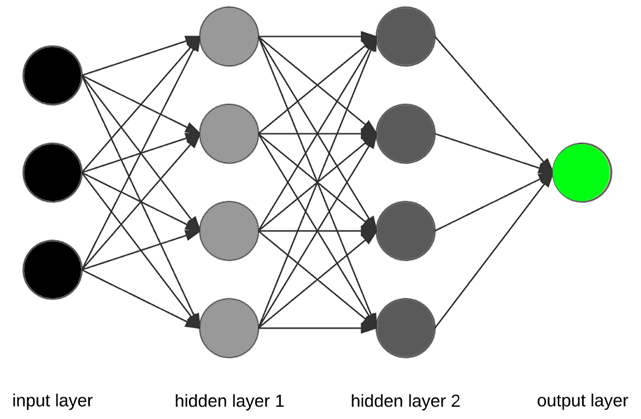
\includegraphics[scale=0.3]{intro.png}}
\caption{Convolutional Layer Between Input and Output Layers}
\label{fig}
\end{figure}

\noindent Meanwhile the models are being used to calculate the accuracy for comparison purposes. The significant contributions of this thesis are stated as follows:  Our model ResNet50 has achieved the highest score among the other models with a validation accuracy of 94.7\%. Moreover, VGG-19 and ResNet50 were the Good-Fit than the other models. However, Glaucoma is one of the leading causes of blindness for people over the age of 60. Statistics show that even with the treatment 15\% to 20\% of patients become blind. For this reason, in this research, we are going to apply Explainable AI to detect Glaucoma in a better way than exists. As the diagnosis of glaucoma is a complicated and expensive process, the application of a Deep Neural network leveraging XAI can give more improvement in understanding or detecting many problems related to glaucoma disease.

\section{Background}

The primary focus of this research is to detect glaucoma at an early stage. Glaucoma is a very common group of eye diseases caused by damage to the optic nerve that connects the eye to the brain and if untreated, it causes permanent loss of vision. It is the second most popular cause of blindness globally. As per experiments, it is tracked down that the conclusion of the experts or ophthalmologists is abstract. This may cause a few misinterpretations when the glaucoma is distinguished as inaccurate, for example, false-positive and false-negative cases. Likewise, glaucoma is asymptomatic in the beginning phase. The harm advances gradually and it has no manifestations or early admonition signs until the vision is lost in the later stage. Additionally, if it tends to be distinguished in the beginning, the visual sight will be saved. It is shown that treatment and standard tests can forestall vision misfortune in individuals just at a beginning phase. On the other hand, if the vision loss has already occurred, the treatment can delay or hinder further vision loss [4]. As it is becoming a big problem day by day that is why research on early detection of glaucoma has gained a massive focus of  the researchers. 

\noindent There are mainly two types of glaucoma. Primary glaucoma also called chronic glaucoma is caused by prolonged intraocular pressure in the eye whereas secondary glaucoma is caused by sudden events such as an injury to the eye or inflammation in the eye or the use of steroids. Both primary and secondary glaucoma can be further classified as open-angle glaucoma and closed-angle glaucoma. Open-angle glaucoma is the most common form of glaucoma and is responsible for 90\% of the cases [5].  In open-angle glaucoma, there is a wide and open angle between the cornea and iris. But in the case of closed-angle glaucoma, the angle is much narrower. Each of these subdivisions can be further divided into classes depending on conditions such as acute, intermittent, chronic, post status, etc. And there are other minor variants of glaucoma such as pigmentary glaucoma, exfoliation glaucoma, primary juvenile glaucoma, etc. In traditional cases, Ophthalmologists use Optical Coherence Tomography or OCT for detecting Glaucoma. Optical Coherence Tomography or OCT is generally utilized for clinical imaging methods. OCT is an optical sign procurement and preparation strategy that catches optic pictures in a three-dimensional picture. Both OCT and ophthalmologists are having a similar issue which is lacking and costly. They must be found in enormous emergency clinics or private emergency clinics. Some glaucoma patients are deficient assets. This can make patients seek a late glaucoma treatment and be awful for their eye wellbeing. The requirement for specialists and a lot of costs are constraints of potential in mass evaluating for early discovery. To take care of the issue of OCT pictures, fundus im-ages are chosen to be input pictures for this venture. A fundus camera is one more sort of camera that can be utilized to catch retina pictures. Fun-dus cameras have more affordable costs for contrasting and OCT pictures. It may very well be found in each region's clinical focus, not just enormous clinics like OCT. Fundus pictures can be utilized for glaucoma finding through the CDR strategy [6].

\noindent Since glaucoma is such a prominent reason for blindness around the world, we must apply our knowledge of classification techniques to classify the various types of glaucoma for the betterment of the world. 

\noindent However, we are portraying and evaluating Convolutional Neural Organization (CNN) models for the discovery of glaucoma dependent on Optical Coherence Tomography (OCT) Retinal Nerve Fiber Layer (RNFL) likelihood maps. Such CNN models can work in pairs with human specialists to keep up with large eye health and assist recognition of visual deficiency causing eye sickness [7]. We can easily use binary classifiers to differentiate between images of primary glaucoma and secondary glaucoma and then we can use another binary classifier to differentiate between images of open-angle glaucoma and closed-angle glaucoma. In this study, we are going to use Explainable AI (XAI) to classify scanned images of eyes that have glaucoma or have the chances to affect in future.

\section{Literature Review}
Glaucoma is one of the most common causes of permanent blindness around the world, from the article [8]. As when the pressure inside the eye is too high in a particular nerve that moment glaucoma will develop and it will also create eye ache. The working mechanisms of the different diagnosis tools like tonometers, gonioscopy, scanning laser tomography, etc are available for the treatment and detection but there are some advantages and disadvantages which sometimes create boundaries. For this, there should be an evaluation of how this works. But with using deep learning the boundaries can be removed. As the XAI concept can be understood by humans which will be closer to the human brain to understand. 

\noindent Another recent similar work, which mentioned Computer-aided diagnostics(CADx) tools, is still struggling to detect glaucoma eye illness according to author Qaisar Abbas [9]. Glaucoma is the main reason for visual disabilities in the whole world. His writings revealed that the Softmax linear classifier makes the ultimate judgment to distinguish between glaucoma and non-glaucoma retinal fundus images. Glaucoma-Deep, the suggested method, was evaluated on 1200 retinal pictures gathered from publicly and privately available datasets. Then the sensitivity (SE), specificity (SP), accuracy (ACC), and precision (PRC) statistical measurements were used to evaluate the performance of the Glaucoma-Deep system. In general, the SE of 84.50\%, SP of 98.01\%, ACC of 99\%, and PRC of 84\% values were achieved through this. When compared to other systems, the Nodular-Deep approach produced much better outcomes. As a result, the Glaucoma-Deep system can quickly identify glaucoma eye illness, solving the problem of clinical specialists during large-scale eye-screening processes. 

\noindent In another recent work we found out that Glaucoma is the leading cause of blindness in the world, and there is no treatment [10]. If it is not diagnosed at an early stage, it can surely lead to irreversible blindness. If vision loss is detected early enough, there are treatments available to prevent it. Because it is a significant chronic eye condition that leads to irreversible blindness. Glaucoma has been on the rise in recent years. Faults in the nerve fiber layer of the retina are diagnosed before apparent abnormalities at the head of the optic nerve and defects in the visual field when 40 percent of axons have been irreversibly destroyed. According to the World Health Organization (WHO) and the World Association of Glaucomatologists (WGO), 66.8 million individuals worldwide suffered from glaucoma in 2010, with 6.7 million becoming blind as a result of the disease.

\noindent Another version of the deep-learning (DL) algorithm was developed in [4] to detect glaucoma disease through extracting several parameters such as 52 total deviation, mean deviation, and pattern standard deviation values. Here the writer used a Deep learning classifier such as a deep feed-forward neural network (FNN). The authors, on the other hand, integrated their DL classifier with older machine learning classifiers including random forests (RF), gradient boosting, support vector machine, and neural network (NN). As a result, the authors provided a deep ensemble solution for glaucoma illness detection. A deep FNN classifier was used to get 92.5 percent of the AUC value, according to the authors. 

\noindent One more research was done from which We learned The impact of artificial intelligence in the diagnosis and management of glaucoma from [11]. Computerized automated visual field testing represents a significant improvement in mapping the island of vision, allowing visual field testing to become a cornerstone in diagnosing and managing glaucoma. Goldbaum developed a two-layer neural network for analyzing visual fields in 1994 et al.[6]. This network classified normal and glaucomatous eyes with the same sensitivity (65\% ) and specificity (72\% ) as two glaucoma specialists. 

\noindent The pathogenesis of glaucoma appears to be dependent on several interconnected pathogenetic mechanisms, including mechanical effects characterized by excessive intraocular pressure, reduced neutrophil produce, hypoxia, excitotoxicity, oxidative stress, and the involvement of autoimmune processes, according to new evidence [12]. Hearing loss has also been linked to the development of glaucoma. In normal tension glaucoma patients with hearing loss, antiphosphatidylserine antibodies of the immunoglobulin G class were shown to be more prevalent than in normal-tension glaucoma patients with normacusis. The World Health Organization reports that glaucoma affects approximately 60 million people worldwide. By the year 2020, it is expected that approximately 80 million people will suffer from glaucoma, which is anticipated to result in 11.2 million cases of bilateral blindness [13]. This is why it needs to be treated as early as possible according to the authors. 

\section{Methodology}

\subsection{Work Plan}
We will use Deep Learning or FCNNs in our work which is a BlackBox function. Generally, Black boxes work excellently but their structure won’t give you any insights that will explain how the function is being approximated. For this, we will use LIME which is one of the most popular XAI-based python libraries. There are a lot of XAI frameworks that explain the BlackBox model’s insights by features. XAI functions work well in terms of explaining complex classification models. In short, these functions generate an explanation through charts of graphs for a complex model's prediction which are also pretty fast. In Figure 4.1 we will see how black boxes work.

\begin{figure}[hbt!]
\centerline{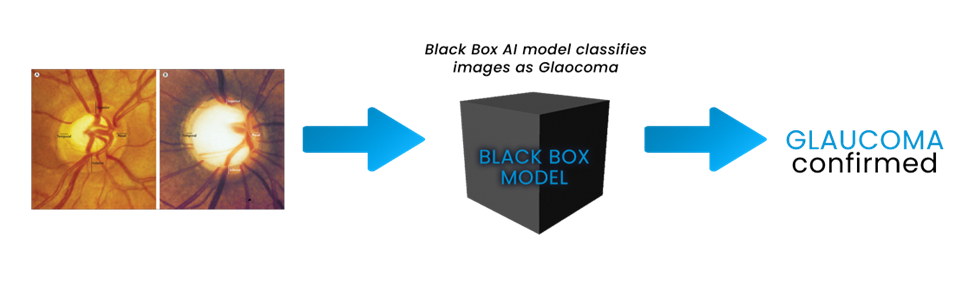
\includegraphics[scale=0.5]{fig-1.png}}
\caption{Blackbox models confirming glaucoma through images}
\label{fig}
\end{figure}

\noindent In Figure 2 we will see how black boxes actually work with the help of lime.

\begin{figure}[htbp]
\centerline{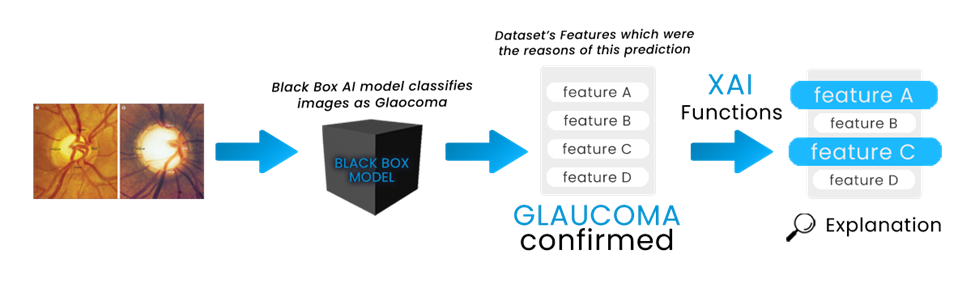
\includegraphics[scale=0.5]{fig-2.png}}
\caption{Blackbox models decision making explanation through LIME}
\label{fig}
\end{figure}

\noindent Here we can see BlackBox models generate a result or output based on some features from the given/training datasets. And through lime, we can have a visualization from which features the output was based on.
In our Glaucoma dataset, we have some features for Suspicious glaucoma and Non-glaucoma. In both sections, we have fundus images, and labels as 1 as the confirmed glaucoma case and 0 as the Non-glaucoma case. To apply XAI, we took Fully Connected Neural Networks (FCNNs) as a black box AI model to predict glaucoma with the help of the data. To compile all of these classifications and determine the average of these scores to one single output, we will use ReLU non-linear activation function in the convolutional layers and the Softmax activation function in the output layers. Below a short rendition is being given for the above Deep Learning models.

\begin{itemize}
  \item \textbf{Convolutional Neural Network (CNN)}: In deep learning, a convolutional neural network (CNN, or ConvNet) is a class of deep neural networks, most commonly applied to analyze visual imagery. We will classify the image data through this model.

  \item \textbf{Fully Connected Neural Network (FCNNs)}: Fully connected neural networks (FCNNs) are a type of artificial neural network where the architecture is such that all the nodes, or neurons, are in one layer, are connected to the neurons in the next layer [14]. This model will also help us to predict and output.

  \item \textbf{ReLU}: A rectified linear activation unit, or ReLU for short, is a node or unit that implements this activation function. Often, networks with hidden layers that use the rectifier function are referred to as rectified networks. The computational cost of adding more ReLUs increases linearly as the size of the CNN grows.

  \item \textbf{Softmax}: Softmax is a mathematical function that transforms a vector of integers into a vector of probabilities, with the probability of each value proportional to the vector's relative scale. The softmax function is most commonly used as an activation function in a neural network model in applied machine learning. The network is set up to produce N values, one for each classification task class, and the softmax function is used to normalize the outputs, turning them from weighted sum values to probabilities that total to one. Each value in the output of the softmax function is interpreted as the probability of membership for each class. This will compile all the convolutional layers of the FCNNs into a single output.
\end{itemize}

\noindent According to our Dataset, we will divide the data chronologically into training and testing data to classify glaucoma.. And through Lime, a XAI function, we will explain these black boxes.

\begin{figure}[hbt!]
\centerline{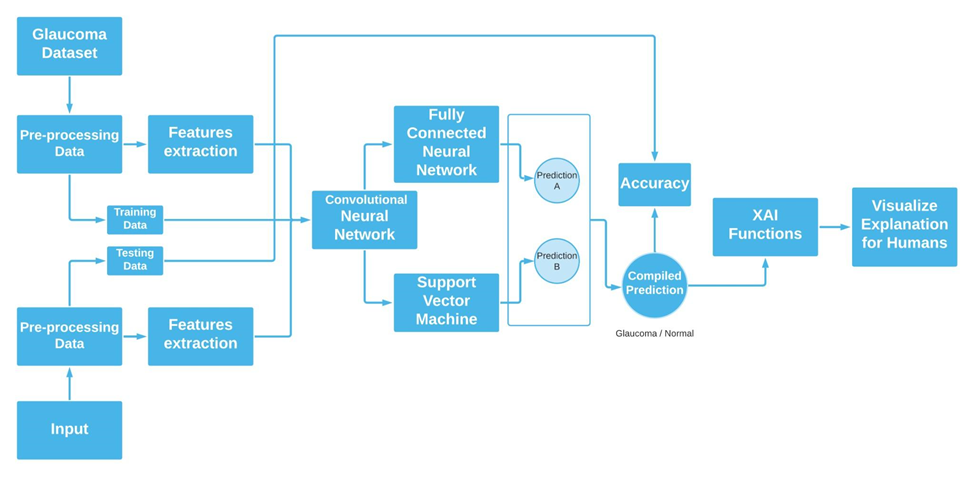
\includegraphics[scale=0.5]{fig-3.png}}
\caption{Work plan of the whole project}
\label{fig}
\end{figure}

\noindent Here in \textbf{[Figure 4]}, we have shown the whole process from dataset preprocessing to compiled output through Softmax activation function. And with XAI functions, we will explain the black boxes through visualization charts of the used core features which were the main reasons behind the prediction.

\subsection{Dataset, Libraries \& Tools}

\noindent As our data are mostly direct fundus images from LAG-Dataset [15]. CNN is being used in this thesis for image classification, as it is a type of model which processes data such as images. Also, it automatically understands low-to high-level patterns of image classification. which helps us to extract higher representations for the image content.

\begin{figure}[hbt!]
\centerline{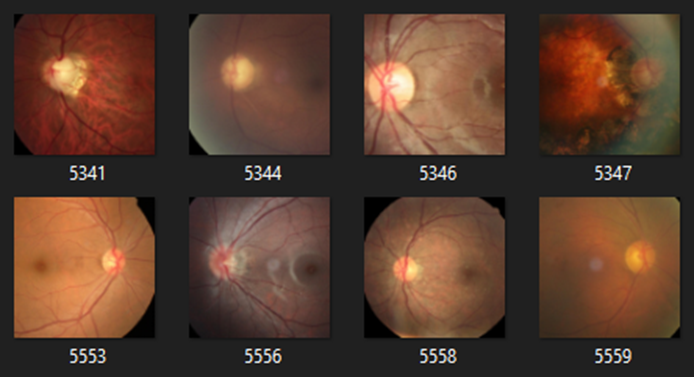
\includegraphics[scale=0.5]{fig-5.png}}
\caption{Sample Data form LAG-Dataset}
\label{fig}
\end{figure}

\noindent This dataset contains 4250 images for training, 302 images for testing and 302 images for validation. All of these images have separated into two folders for glaucoma and non glaucoma. The label for “glaucoma” is 1 and for “non-glaucoma” is 0.

\begin{table}[hbt!]
\begin{align}
\resizebox{1cm}{!}{\textwidth}{%
\begin{tabular}{|c|c|c|}
\hline
Class               & Label & Fundus Image \\ \hline
Suspicious Glaucoma & 1     & 1711         \\ \hline
Non Glaucoma        & 0     & 3143         \\ \hline
\end{tabular}%
}
\end{align}
\end{table}


\subsection{Architecture}
In deep learning, a convolutional neural network (CNN, or ConvNet) is a class of artificial neural networks, most commonly applied to analyze visual imagery[20]. In this study, a Transfer Learning approach is proposed. The data set’s size and features provide a perfect environment for implementing a transfer learning approach, allowing a pre-trained CNN with all of its weights to be utilized to develop a new transfer learning model specialized to identifying Glaucoma with a high degree of accuracy. 

\noindent We used pre-trained models from Tensorflow Keras implementation and through Transfer Learning we trained only the layers we need to train. All the model's weights were trained from the ImageNet dataset. After downloading the pre-trained model we have made every trained layer into untrainable layers and deleted the top layers to reuse the model. Then we use a Flatten layer to flatten every pre-trained layer of the keras model's into one and we used 3 Dense neurons with 100 layers in each of it for VGG-16, VGG-19, InceptionV3 and ResNet50. For DenseNet121 we used 1024 layers for first, 512 layers for second and 256 layers for third neuron. We used the “ReLU” activation function for the Convolutional layers. We also performed batch normalization and a dropout with the rate of 0.5 in each model. For predictions, we used the A Dense neuron with 2 layers in it and “Softmax” for activation function. For the Gradient Descent, we used the Adam optimizer with a learning rate of 1-e^{−5}.

\begin{figure}[hbt!]
\centerline{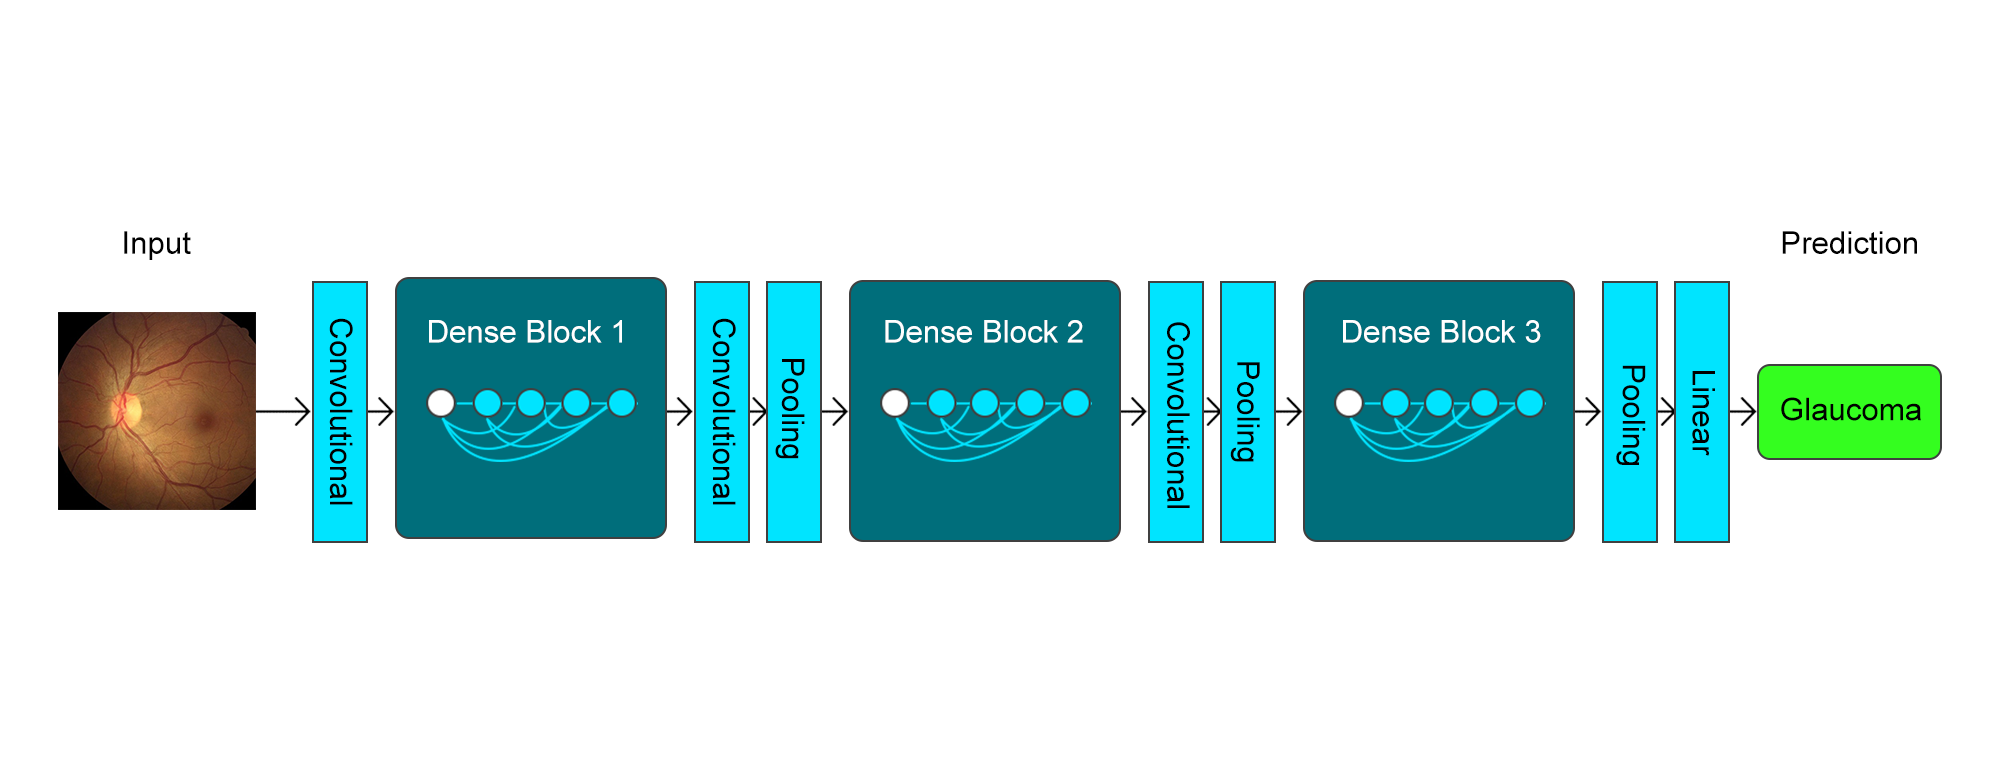
\includegraphics[scale=0.25]{densenet archinew.png}}
\caption{Architecture of DenseNet121}
\label{fig}
\end{figure}


\begin{figure}[hbt!]
\centerline{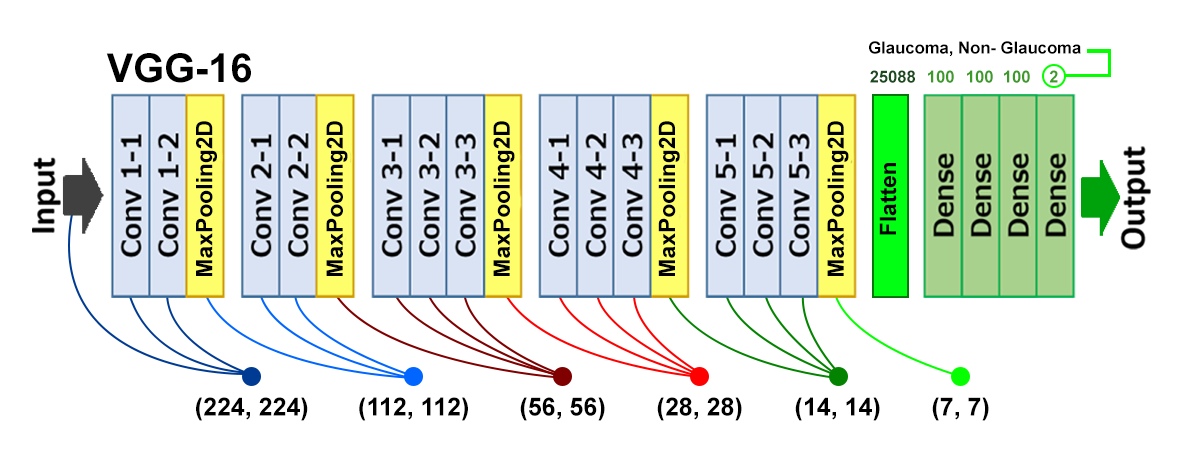
\includegraphics[scale=0.4]{vgg16 architecture.png}}
\caption{Architecture of VGG-16}
\label{fig}
\end{figure}


\begin{figure}[hbt!]
\centerline{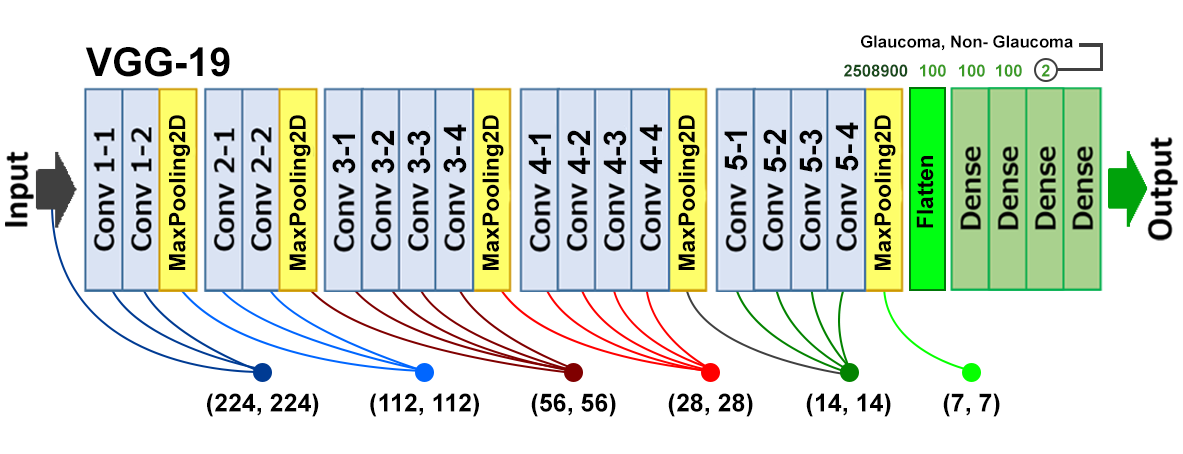
\includegraphics[scale=0.4]{vgg19archireal.png}}
\caption{Architecture of VGG-19}
\label{fig}
\end{figure}


\begin{figure}[hbt!]
\centerline{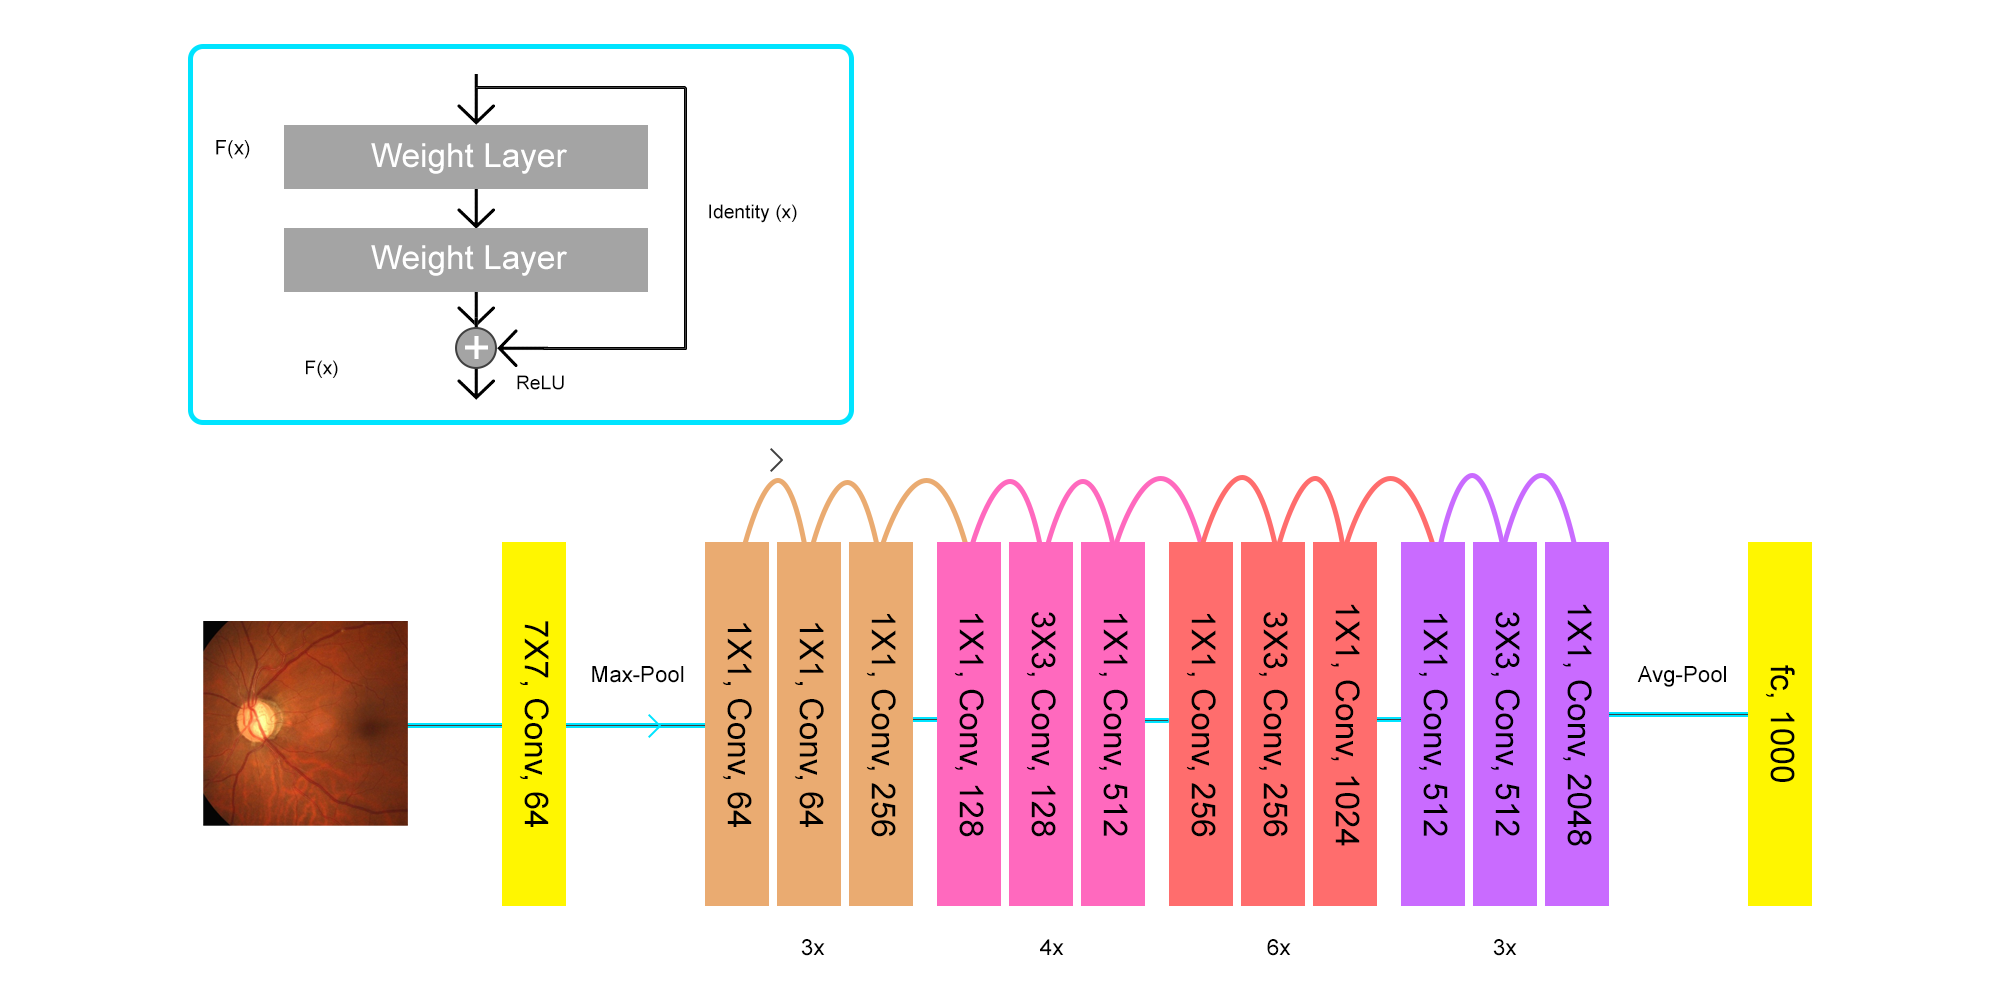
\includegraphics[scale=0.3]{resnet50.png}}
\caption{Architecture of ResNet50}
\label{fig}
\end{figure}

\subsection{Transfer Learning \& Fine Turing}

In deep learning, a convolutional neural network (CNN, or ConvNet) is a class of artificial neural networks, most commonly applied to analyze visual imagery [13].
In this study, a Transfer Learning approach is proposed. The data set’s size and features provide a perfect environment for implementing a transfer learning approach, allowing a pre-trained CNN with all of its weights to be utilized to develop a new transfer learning model specialized to identifying Glaucoma with a high degree of accuracy. We are going with the Fine-Tuning approach of Transfer Learning.

\noindent Fine-tuning is the process of fine-tuning or changing a model that has already been trained for one task to make it execute a second related task. A deep learning network that recognizes cars, for example, maybe fine-tuned to recognize trucks [16]. As proposed, we will be using Fine-tuning approach to detect Glaucoma from our dataset which will help to detect our wanted result in this study.

\subsection{Convolutional Operation}
As illustrated in figure 5.15, the convolutional layers are responsible for convolution operations. It produces feature maps that learn the features of the image taken as input by convolving correctly learnt filters or kernels with the input array or tensor. From the early layers to the distant edging layers, a convolution operation has a number of feature maps that gather new features and respond to feature hierarchy throughout the neural network.[29][34][30

\begin{figure}[hbt!]
\centerline{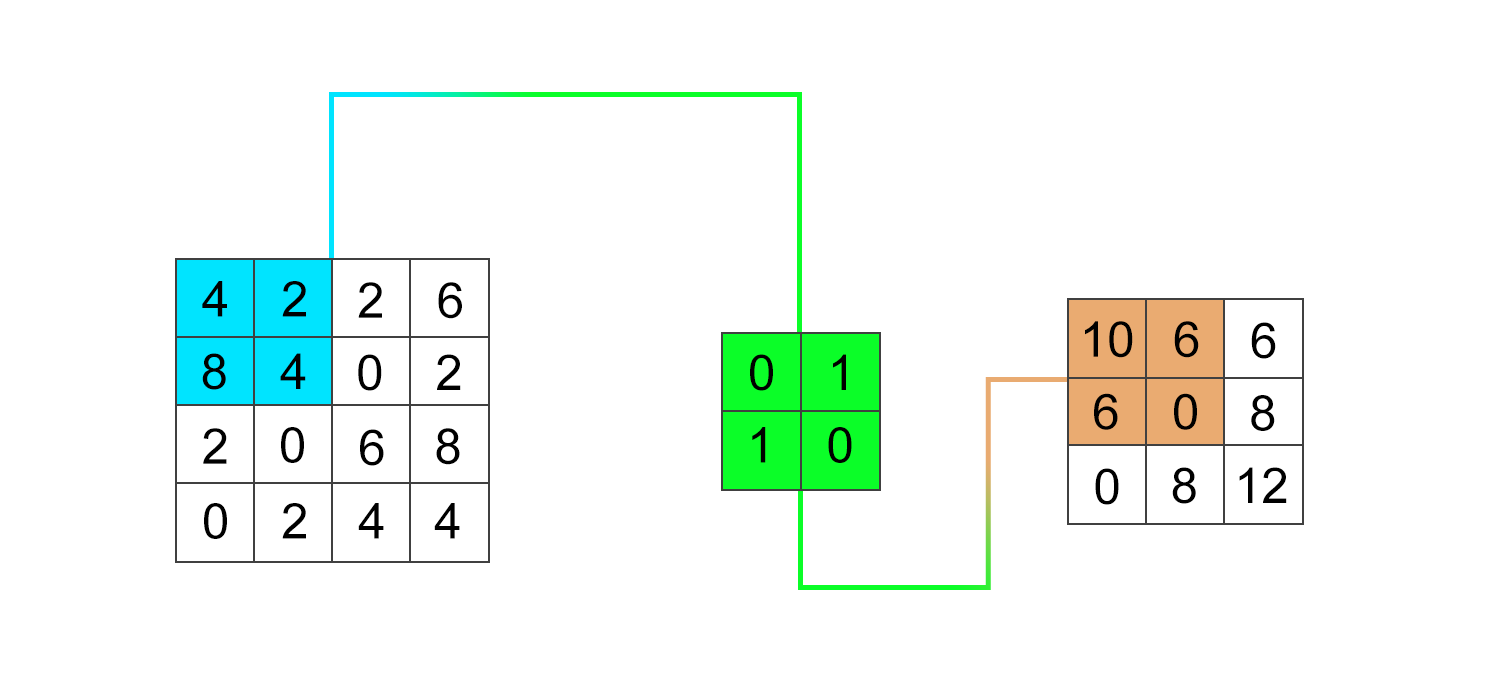
\includegraphics[scale=0.4]{feature map.png}}
\caption{Convolution Operation}
\label{fig}
\end{figure}

\noindent To extract additional features and reduce their dimension, the feature maps are concatenated.[30]. In general, the pooling operation is carried out as follows:

\begin{figure}[hbt!]
\centerline{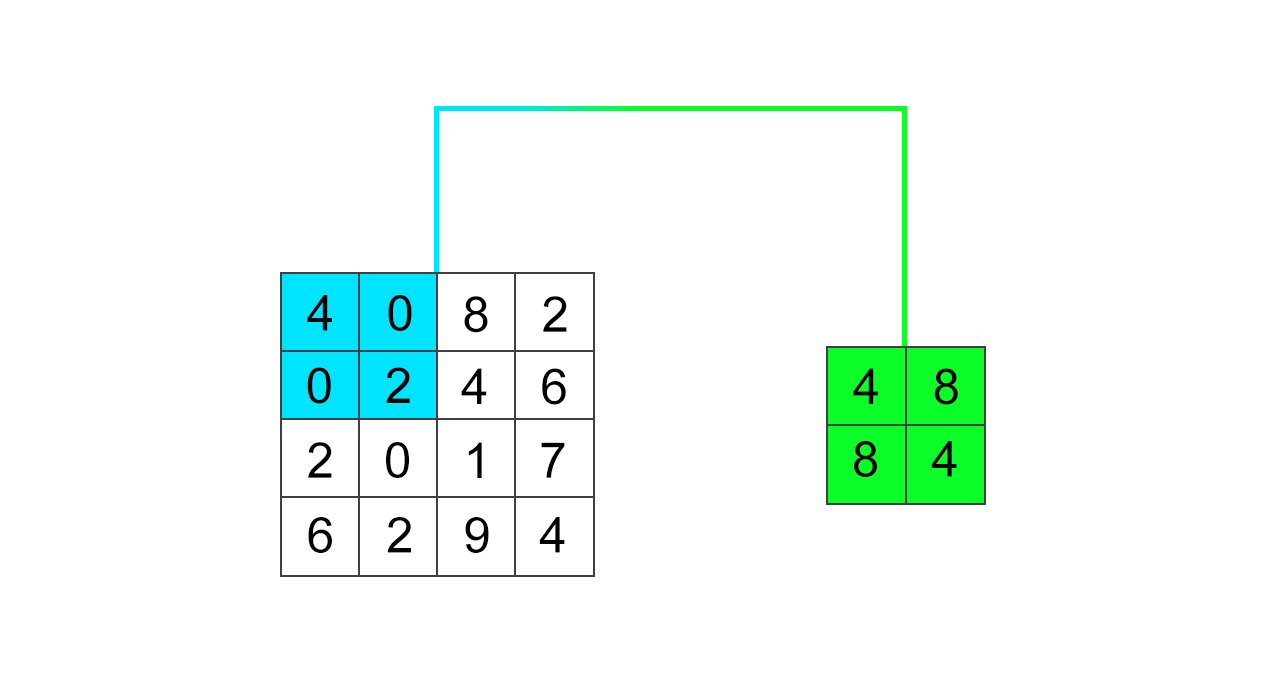
\includegraphics[scale=0.4]{pooling.png}}
\caption{Pooling Operation}
\label{fig}
\end{figure}

\subsection{Optimization Algorithm}

When deep learning is utilized for training, an optimization technique is applied to improve the cost function. This algorithm’s general equation is as follows:

\begin{equation*}
J(W,\ b) = \frac{1}{m}\sum_{i=1}^m\ L(y^{'i},y^i)
\end{equation*}

\noindent In our model, we used Adam optimizer which is explained below: Adam is a well-
known algorithm that is noted for its speed. Adaptive Momentum is the abbreviation for AdaM. At the same time, Adam associates the propulsion RMSprop. As a result, Adam is a highly powerful and quick algorithm. This approach is relatively straightforward in its implementation, quite efficient in estimate, and uses very little memory. For larger issues with data or parameters, it is more efficient. The optimizer is defined by the equations below:

\begin{equation*}
\begin{split}
\alpha_t = \alpha.\frac{\sqrt{1-\beta^t_2}}{1-\beta^t_2} \\
\theta_t\leftarrow\theta_{t-1}-\alpha_t-.m_{\frac{t}{(\sqrt{v_t}+\hat{\epsilon})}}
\end{split}
\end{equation*}

\noindent For the Gradient Descent, we used the Adam optimizer with a learning rate of 10-5.

\subsection{Activation Function}

\noindent \textbf{SoftMax:} The output of this function is a probability distribution. As the entire summation becomes 1, it maps the input. This function is defined by the equation given below:

\vspace{5mm}
\begin{equation*}
f_j(z)=\frac{e^{zj}}{\sum_k{e^zk}} 
\end{equation*}

\noindent It takes a vector of arbitrary real-valued scores (in z) and squashes it to a vector of values between zero and one that sum to one.
Rectified Linear Unit (ReLU): ReLU is a piecewise linear function that outputs the provided input directly. It has a 0 to range. In the deep learning era, ReLu is the most well-known activation function, as seen in the equation below:

\vspace{5mm}
\begin{equation*}
y=max(0,x) 
\end{equation*}

\noindent The key benefit of ReLU is that it addresses the vanishing gradient problem, is one-sided (unlike TanH), has sparse activation (50\%) and has no back propagation error. This function is monotonic, as are its derivatives. This function has the disadvantages of being non-zero centered and non-differentiable by zero. Another disadvantage is the dying ReLU problem, which occurs when half of the outputs for non-zero centered action are inactive (returned as 0).

\vspace{5mm}
\section{Implementation}
\subsection{Analysis}
We have used VGG-16, VGG-19, DenseNet121, InceptionV3 and ResNet50 models for our study. Every model was compiled with Adam optimizer with the learning rate of 1e-5 in 50 epochs.
After 50 epochs, RestNet50 got the highest score among the other models with a validation accuracy of 94.7\%.

\noindent These are the Train and Test score of our models -

\noindent In \textbf{Table I}, the Train and Test accuracy and loss graph for each model are given.

\begin{table}[hbt!]
\resizebox{5mm}{!}{\textwidth}{%
\scalebox{0.9}{
\begin{tabular}{|c|c|c|c|c|}
\hline
Model       & Accuracy & Train Accuracy & Train Loss & Validation Loss \\ \hline
DenseNet121 & 86.81\%  & 88.83\%        & 31.18\%    & 24.10\%         \\ \hline
InceptionV3 & 86.42\%  & 93.49\%        & 20.04\%    & 35.79\%         \\ \hline
ResNet50    & 94.71\%  & 99.56\%        & 3.81\%     & 12.22\%         \\ \hline
VGG-16      & 88.63\%  & 98.00\%        & 6.76\%     & 27.92\%         \\ \hline
VGG-19      & 93.31\%  & 97.00\%        & 11.53\%    & 14.94\%         \\ \hline

\end{tabular}%
}
}
\caption{Model Accuracy and Loss}
\label{tab:Model Accuracy and Loss}
\end{table}

\noindent The shape and dynamics of a learning curve can be used to diagnose the behavior of a machine learning model and in turn perhaps suggest the type of configuration changes that may be made to improve learning and/or performance. We know that smaller relative scores on the y-axis indicate more or better learning.

\noindent There are three common dynamics that you are likely to observe in learning curves. And they are Underfit, Overfit and Good Fit.  And by observing the models, VGG19 had the best fit than the others and then the Resnet50. But the DenseNet121 is underfitted as the training loss is over the validation loss. VGG-16 and InceptionV3 got over-fitted as the train loss curve  goes under the value loss curve or on the other hand train accuracy is much higher than the validation accuracy.

\noindent These are the Train sets, True and Predicted scores of classified and misclassified glaucoma and non-glaucoma results for each model based on the model’s train datasets prediction labels and the actual train labels. We have added a threshold of 0.5 for this train predicted visualization.

\noindent\textit{(the percentages are meaning the predicted train accuracy for the predicted labels calculated with the actual train labels)}

\vspace{5mm}
\begin{figure}[hbt!]
\centering
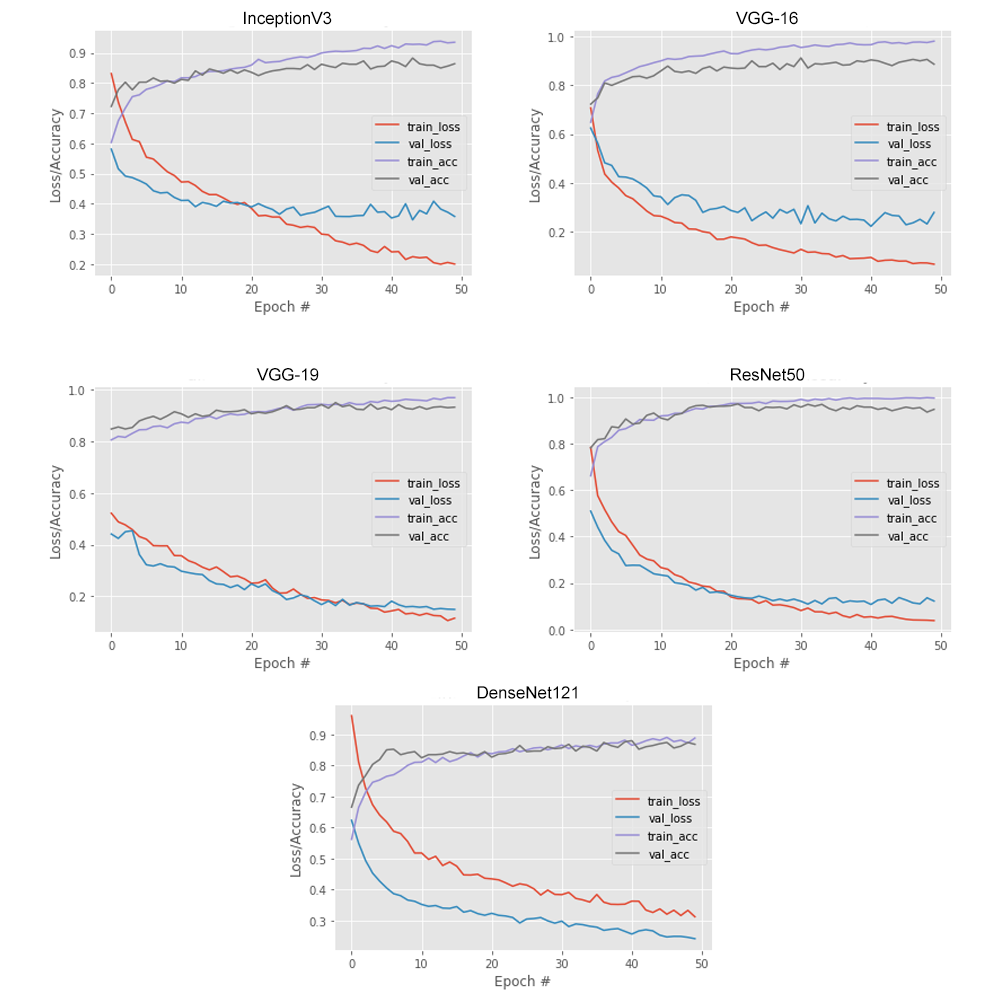
\includegraphics[scale=0.5]{fig-35.png}
\caption{All Model’s Train Test Accuracy and Loss Curve}
\end{figure}

\noindent Comparing All models' Accuracy and Loss graph together, we can see that VGG-19 and ResNet50 were the Good-Fit than the other models.

\noindent These are the Train sets, True and Predicted scores of classified and misclassified glaucoma and non-glaucoma results for each model based on the model’s train datasets prediction labels and the actual train labels. We have added a threshold of 0.5 for this train predicted visualization.

\noindent\textit{(the percentages are meaning the predicted train accuracy for the predicted labels calculated with the actual train labels)}

\vspace{5mm}
\begin{figure}[hbt!]
\centering
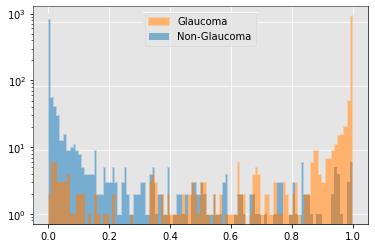
\includegraphics[scale=0.5]{fig-36.png}
\caption{True and Predicted Train scores of DenseNet121}
\label{fig:x True and Predicted Train scores of DenseNet121}
\end{figure}

% \centering
\begin{center}
All  151 misclassified samples (93.83\%) 

Glaucoma  74 misclassified samples (93.95\%)

Non-Glaucoma  77 misclassified samples (93.71\%)
\end{center}
\vspace{5mm}
\begin{figure}[hbt!]
\centering
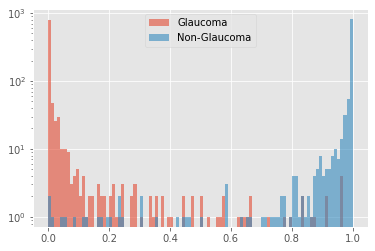
\includegraphics[scale=0.5]{fig-37.png}
\caption{True and Predicted Train scores of InceptionV3}
\label{fig:x True and Predicted Train scores of InceptionV3}
\end{figure}

% \centering
\begin{center}
All   48 misclassified samples (97.65\%)

Glaucoma  22 misclassified samples (97.84\%)

Non-Glaucoma  26 misclassified samples (97.45\%)
\end{center}
\vspace{5mm}
\begin{figure}[hbt!]
\centering
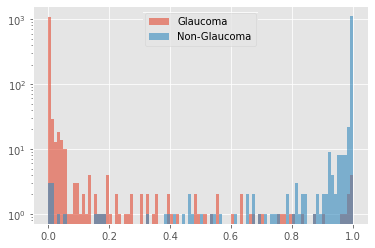
\includegraphics[scale=0.5]{fig-38.png}
\caption{True and Predicted Train scores of VGG-16}
\label{fig:x True and Predicted Train scores of VGG-16}
\end{figure}

% \centering
\begin{center}
\newpage
All   47 misclassified samples (98.08\%)

Glaucoma  20 misclassified samples (98.37\%)

Non-Glaucoma  27 misclassified samples (97.79\%)
\end{center}
\vspace{5mm}
\begin{figure}[hbt!]
\centering
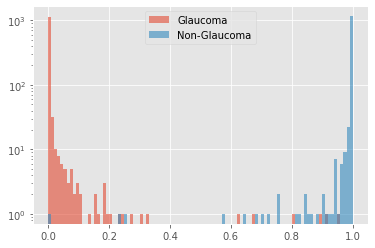
\includegraphics[scale=0.5]{fig-39.png}
\caption{True and Predicted Train scores of VGG-19}
\label{fig:x True and Predicted Train scores of VGG-19}
\end{figure}
\begin{center}
All   17 misclassified samples (99.31\%)

Glaucoma  14 misclassified samples (98.86\%)

Non-Glaucoma   3 misclassified samples (99.75\%)
\end{center}
\vspace{5mm}
\begin{figure}[hbt!]
\centering
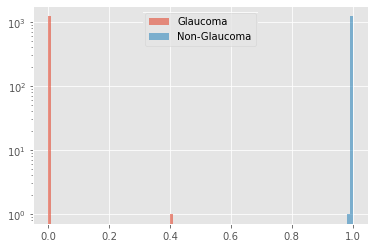
\includegraphics[scale=0.5]{fig-40.png}
\caption{True and Predicted Train scores of ResNet50}
\label{fig:x True and Predicted Train scores of ResNet50}
\end{figure}
\begin{center}
All    0 misclassified samples (100.00\%)

Glaucoma   0 misclassified samples (100.00\%)

Non-Glaucoma   0 misclassified samples (100.00\%)
\end{center}
\vspace{5mm}
Now, We have called the same function that we have used for the above Train predicted labels again with the same threshold of 0.5. But for now we have used the validation datasets prediction labels. And the results were - 

\noindent \textit{(the percentages are meaning the predicted test/validation accuracy for the predicted labels calculated with the actual test/validation labels)}

\noindent \textit{( Here, G = Glaucoma and n-G = Non-Glaucoma )}

\begin{center}
\begin{table}[hbt!]
\centering
\begin{tabular}{|p{1.5cm}|p{1.5cm}|p{1.5cm}|c|}
\hline
% \parbox{\centering \textbf{Model}} & \parbox{\centering \textbf{All misclassified}} & \parbox{\centering \textbf{G misclassified}} & \parbox{\centering \textbf{n-G misclassified}} \\

\centering{\textbf{Model} & \centering\textbf{All misclassified} & \centering\textbf{G misclassified} & \textbf{n-G misclassified}} \\
\hline
\centering DenseNet121 & \centering 9 (86.76\%) & \centering 4 (88.24\%) & 5 (85.29\%)\\
\hline
\centering InceptionV3 & \centering 24 (85.88\%) & \centering 16 (81.18\%) & 8 (90.59\%)\\
\hline
\centering VGG-16 & \centering 8 (88.24\%) & \centering 7 (79.41\%) & 1 (97.06\%)\\
\hline
\centering VGG-19 & \centering 4 (94.12\%) & \centering 3 (91.18\%) & 1 (97.06\%)\\
\hline
\centering ResNet50 & \centering 3 (95.59\%) & \centering 1 (97.06\%) & 2 (94.12\%)\\
\hline
\end{tabular}
\caption{True and Predicted Test scores of all Model}
\label{tab:True and Predicted Test scores of all Model}
\end{table}
\end{center}



\vspace{5mm}
\noindent Now we have taken a single predicted batch from each model’s prediction with the 0.5 threshold and plotted the misclassified glaucoma and non-glaucoma images, which we will use in Lime (XAI framework) to explain later.

\noindent \textit{( Here, G = Glaucoma and n-G = Non-Glaucoma )}

\begin{table}[hbt!]
\begin{tabular}{|c | c | c| c |}
\hline
\textbf{Model} & \textbf{Batch} & \textbf{G misclassified} & \textbf{n-G misclassified}}\\
\hline
DenseNet121 & 2 (32 in each) & 3 &  5\\
\hline
InceptionV3 & 2 (32 in each) & 2 & 7\\
\hline
VGG-16 & 2 (32 in each) & 2 & 3\\
\hline
VGG-19 & 2 (32 in each) & 1 & 4\\
\hline
ResNet50 & 2 (32 in each) & 0 & 3\\
\hline

\end{tabular}
\caption{True and Predicted Test scores of all Model}
\label{tab:True and Predicted Test scores of all Model}
\end{table}

\vspace{5mm}
\noindent These are some of the misclassified images for all models with and undoing the existing preprocessing. Basically the model’s preprocessing for these images ruined their actual color and contrast.  Which led the model to predict wrong. By undoing the existing preprocessing we can see that for DesneNet121 the images got a little reddish and for other models, It got bluish.

\begin{figure}[hbt!]
\centering
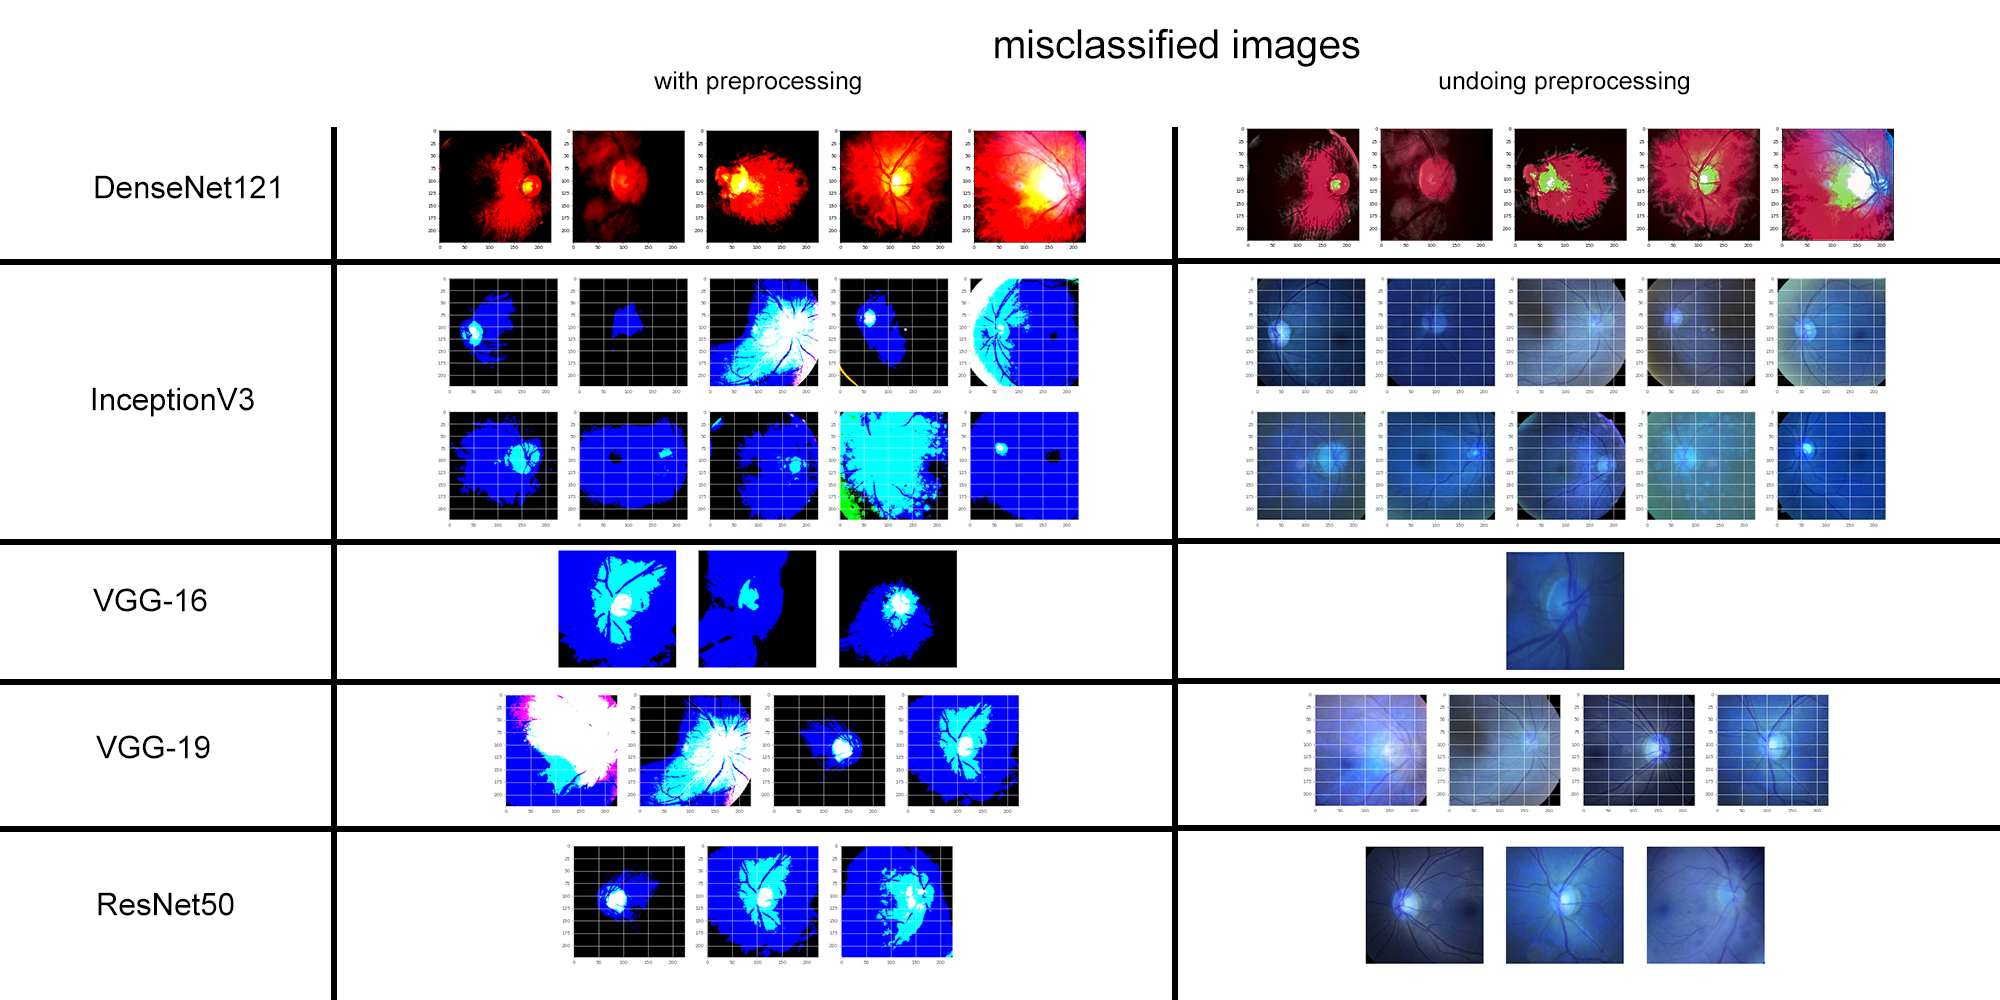
\includegraphics[scale=0.25]{fig-41.png}
\caption{Misclassified images for all models with and without preprocessing}
\label{fig:x True and Predicted Train scores of ResNet50}
\end{figure}

\subsection{Result}
These are the single image predictions of all models - 

\noindent\textit{( here outputs are given in [n,m] format, where “m” means glaucoma score and “n” means non-glaucoma score )}

\begin{figure}[hbt!]
\centering
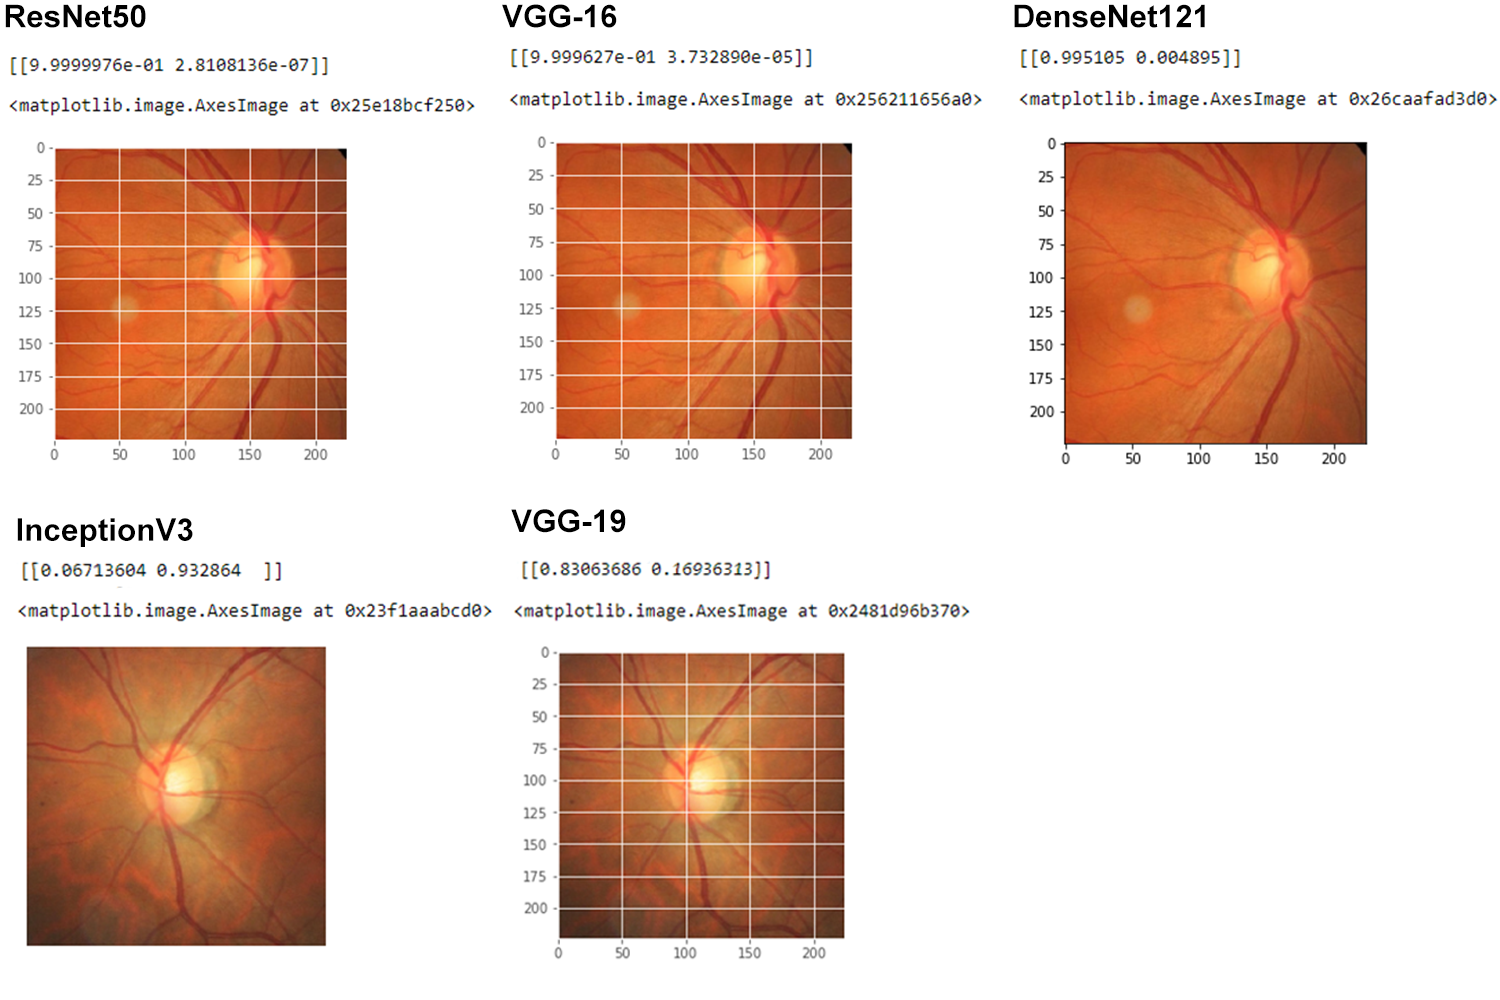
\includegraphics[scale=0.25]{fig-53.png}
\caption{Single Image Predictions for all Model}
\label{fig:x Single Image Predictions for all Model}
\end{figure}



\noindent\textit{These are batch (50 images/batch) image predictions of all models - ( here [1,0] means glaucoma and [0,1] means non-glaucoma )}

\begin{figure}[hbt!]
\centering
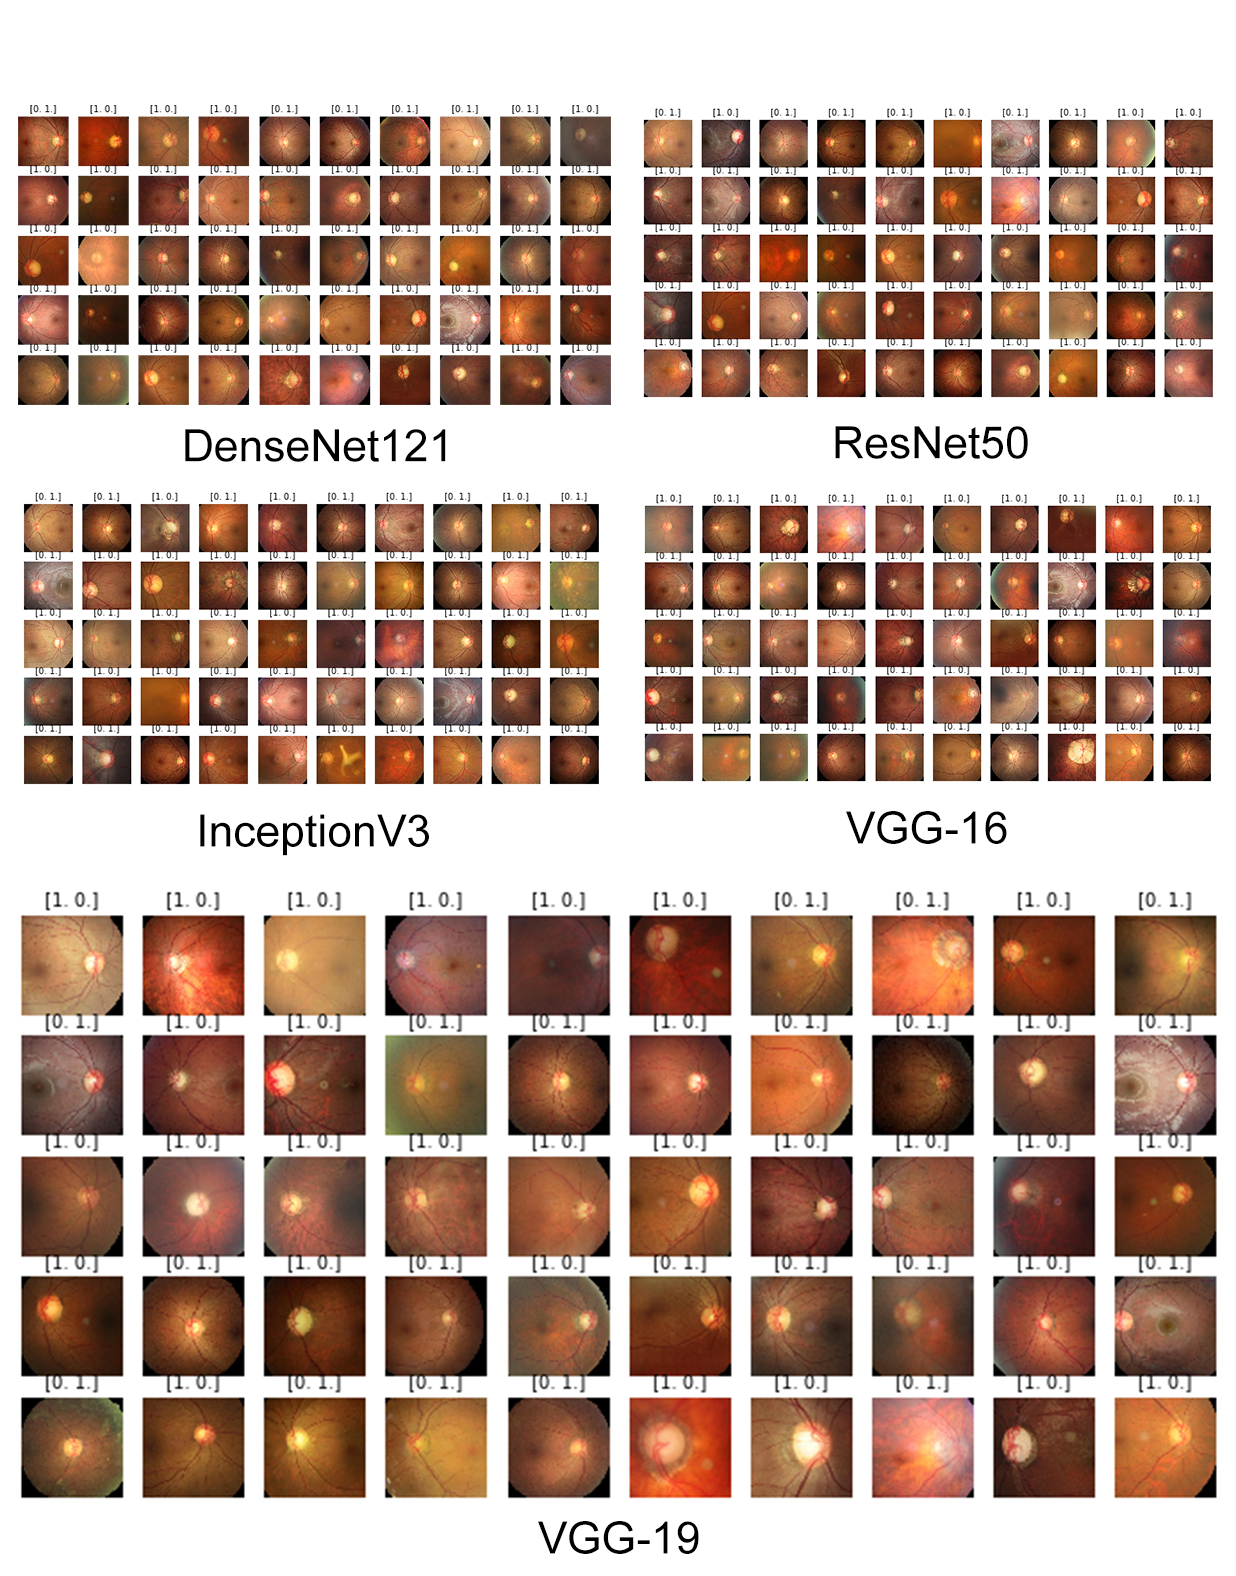
\includegraphics[scale=0.30]{batch prediction.png}
\caption{Batch Predictions for all Model}
\label{fig:x Batch Predictions for all Model}
\end{figure}

\subsection{Applying XAI (Lime)}

 Now we will show the explanation for these preprocessed and misclassified images using an XAI [17] framework, LIME. Then we will apply Lime again on a single predicted raw fundus -image directly from the test dataset (labelled) directory to see the difference between a correctly predicted fundus image [18] and wrong predicted fundus image. Given below are the misclassified image with preprocessing, Superpixels focused area and the model prediction explanation by Lime in DenseNet12.

\noindent LIME stands for Local Interpretable Model-agnostic Explanations which is an explainable AI method. Its goal is to make the predictions of machine learning models understandable to humans. The method can explain individual instances which makes it suitable for local explanations. LIME manipulates the input data and creates a series of artificial data containing only a part of the original attributes. Thus, in the case of text data, for example, different versions of the original text are created, in which a certain number of different, randomly selected words are removed. This new artificial data is then assigned to different categories (classified). Hence, through the presence or absence of certain keywords we can see their influence on the classification of the selected text. LIME gives the output as a list of explanations which reflects the contribution of each feature which resulted in the final prediction.

\begin{figure}[hbt!]
\centering
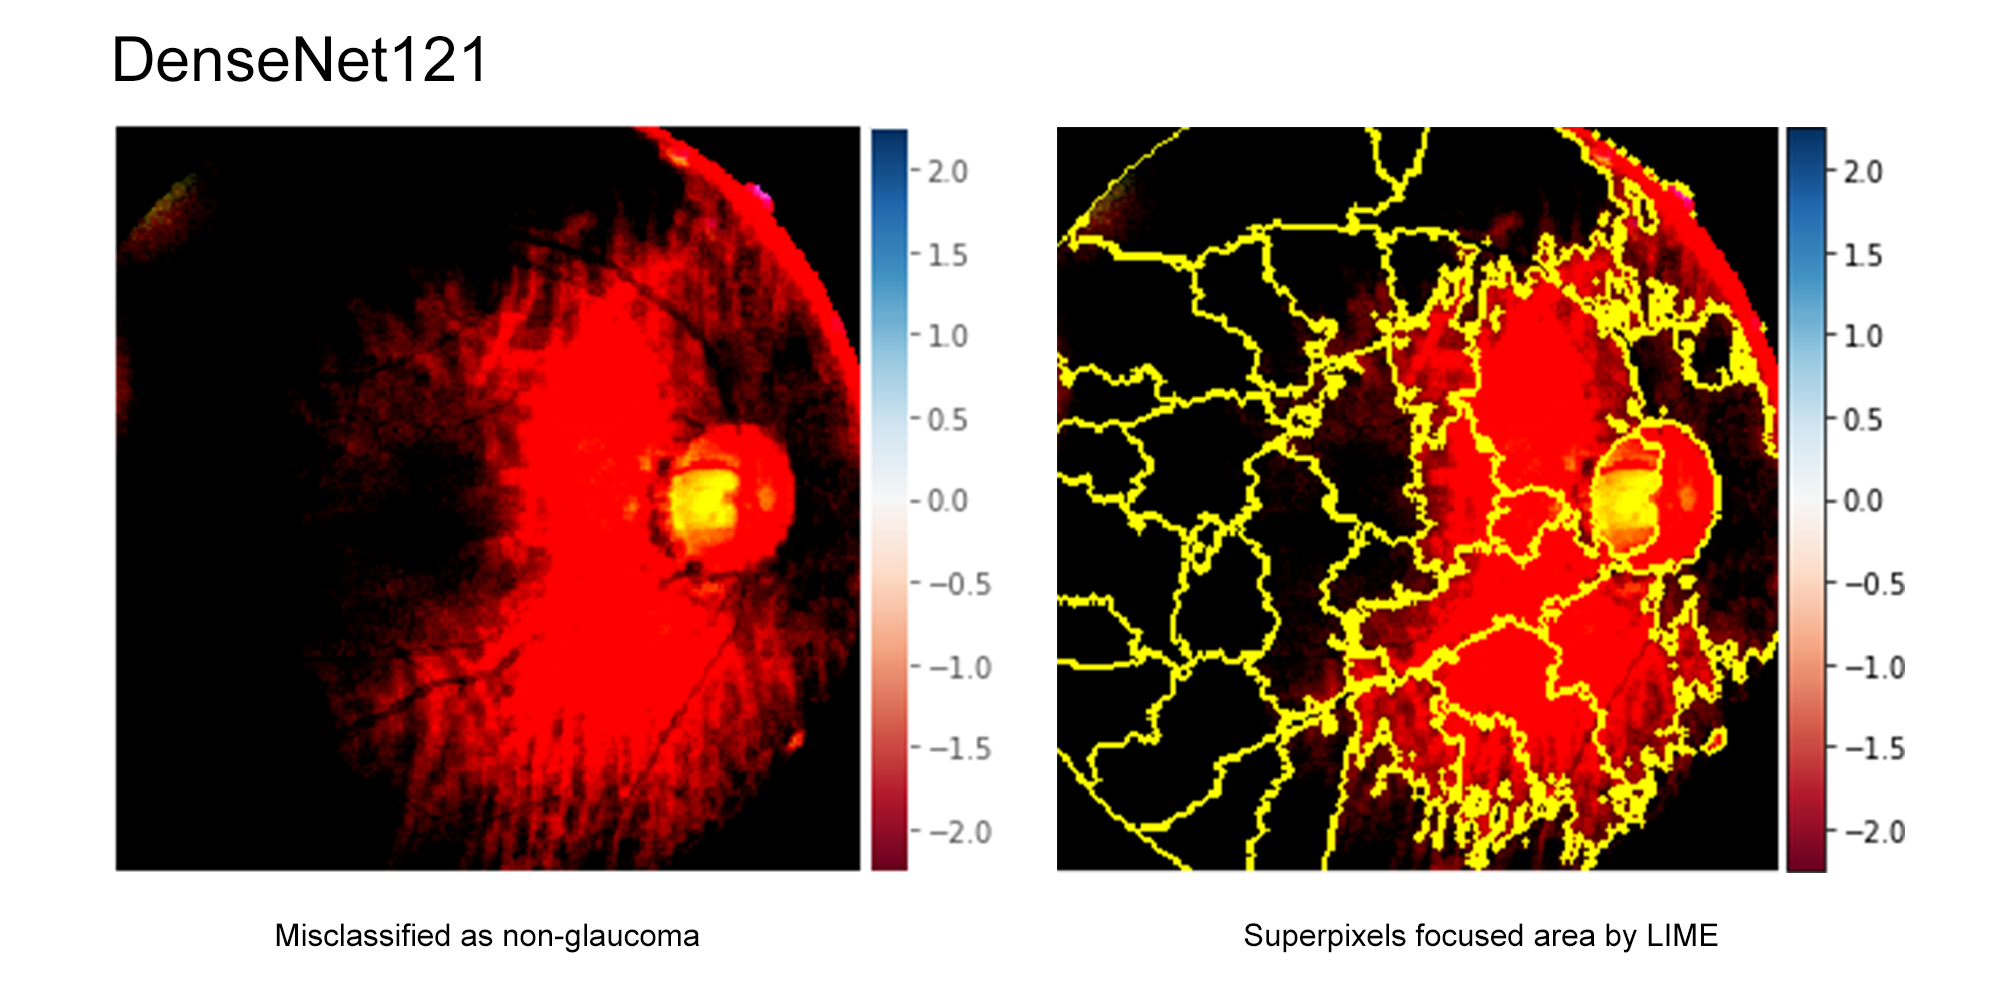
\includegraphics[scale=0.24]{fig-42.png}
\caption{Misclassified image with preprocessing and Superpixels focused area by Lime in DenseNet121}
\label{fig:x Misclassified image with preprocessing and Superpixels focused area by Lime in DenseNet121}
\end{figure}

\begin{figure}[hbt!]
\centering
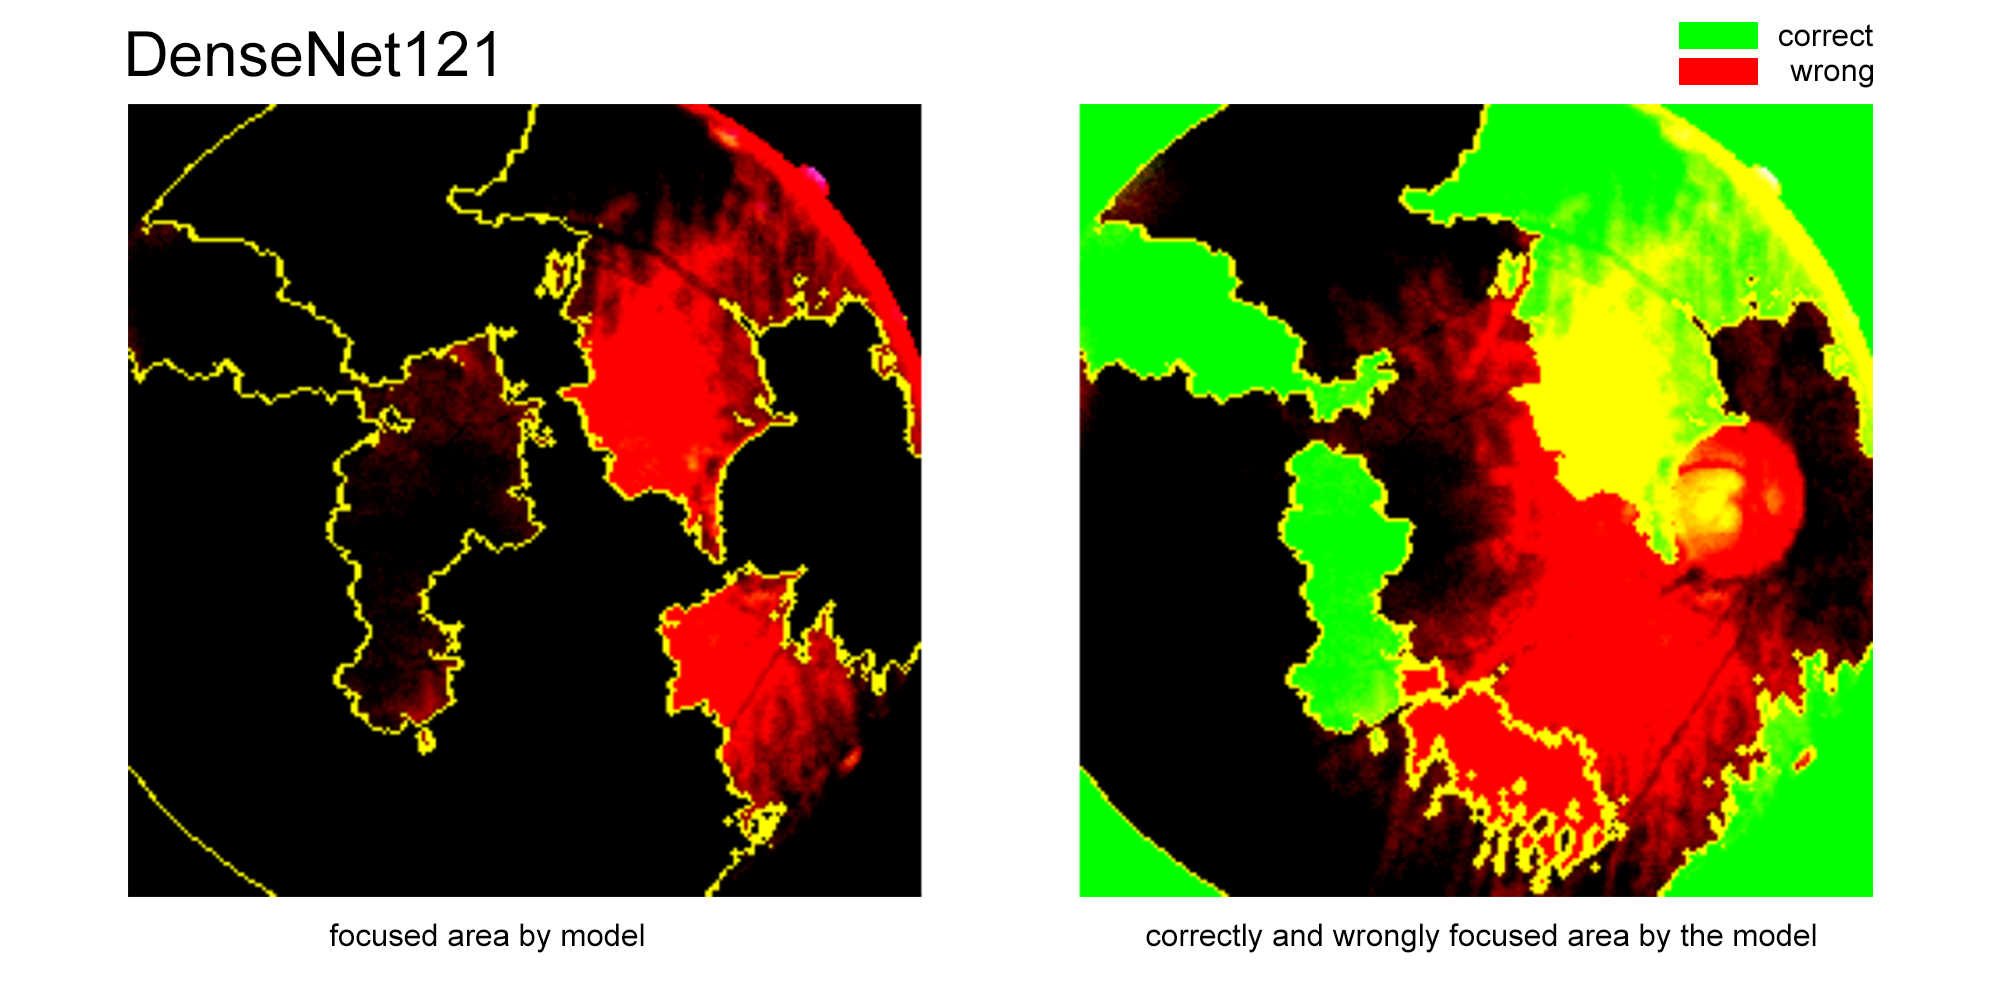
\includegraphics[scale=0.24]{fig-43.png}
\caption{Lime Explanation for DenseNet121}
\label{fig:x Lime Explanation for DenseNet121}
\end{figure}

\begin{figure}[hbt!]
\centering
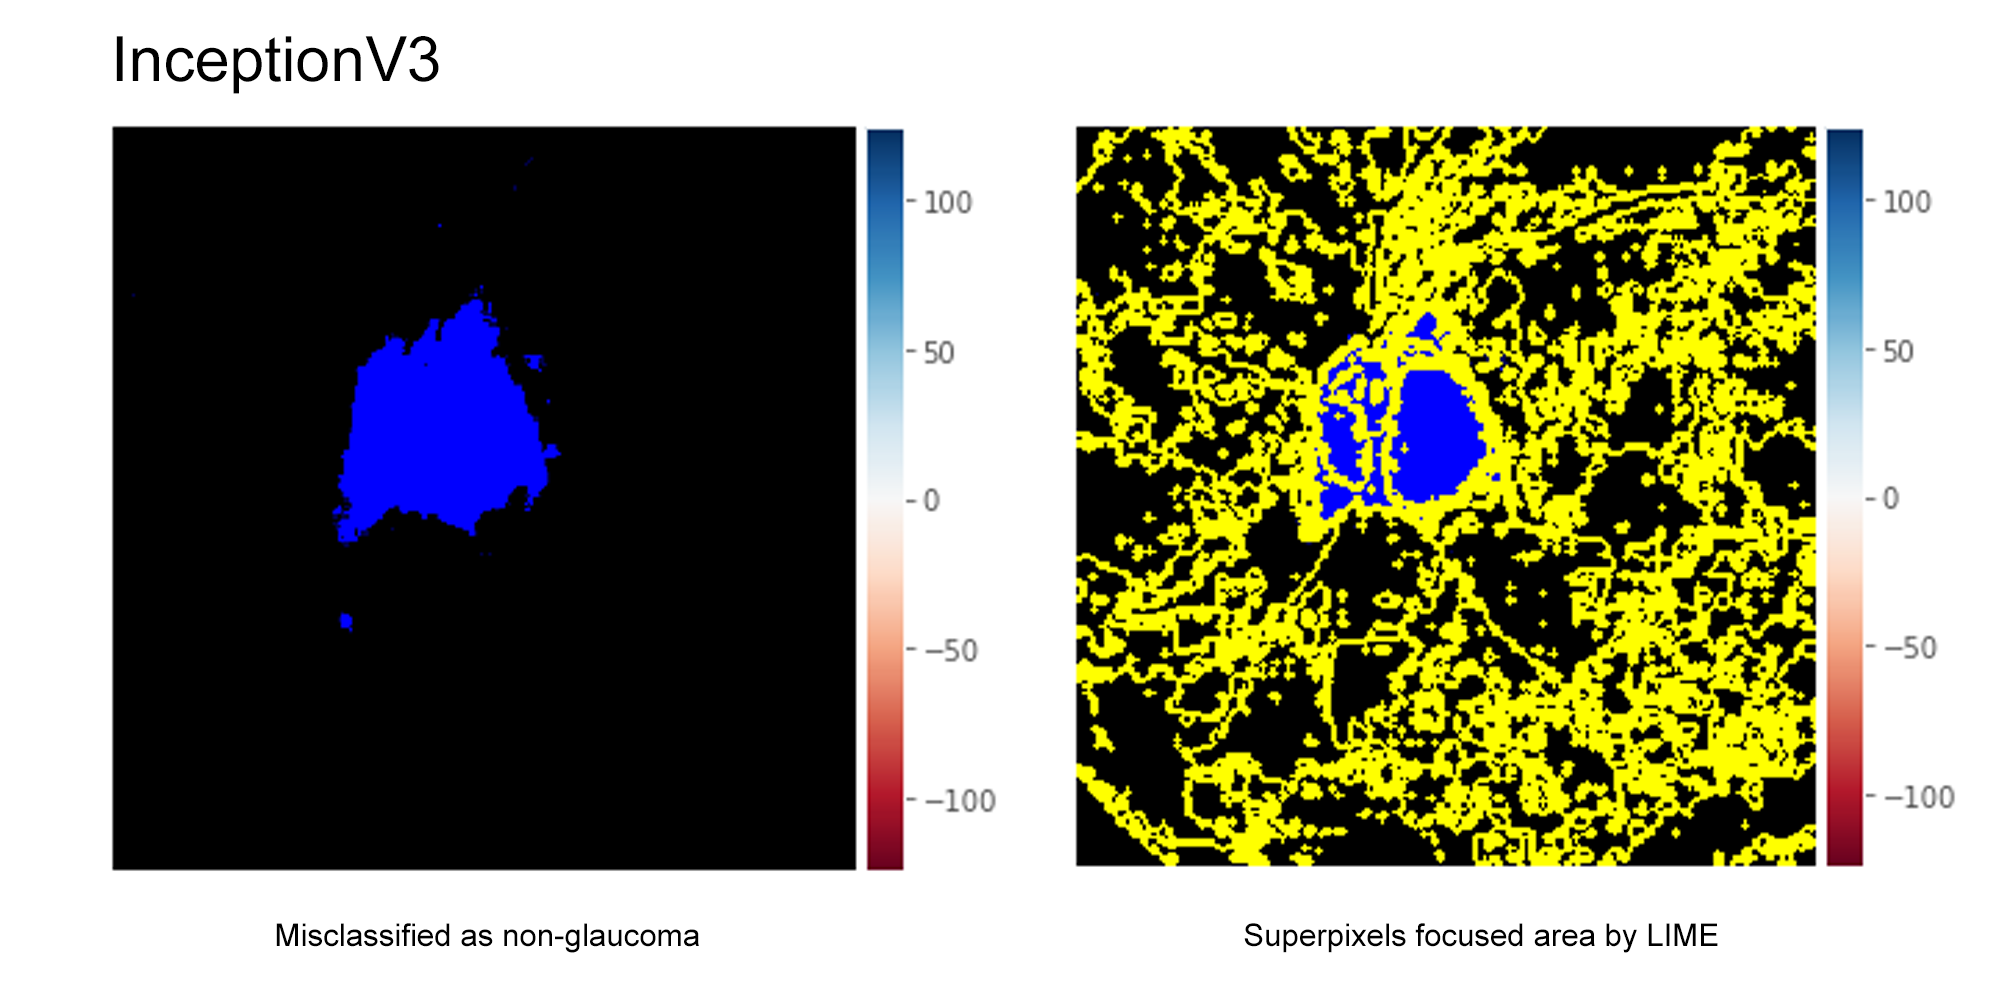
\includegraphics[scale=0.24]{fig-44.png}
\caption{Misclassified image with preprocessing and Superpixels focused area by Lime in InceptionV3
}
\label{fig:x Misclassified image with preprocessing and Superpixels focused area by Lime in InceptionV3
}
\end{figure}

\begin{figure}[hbt!]
\centering
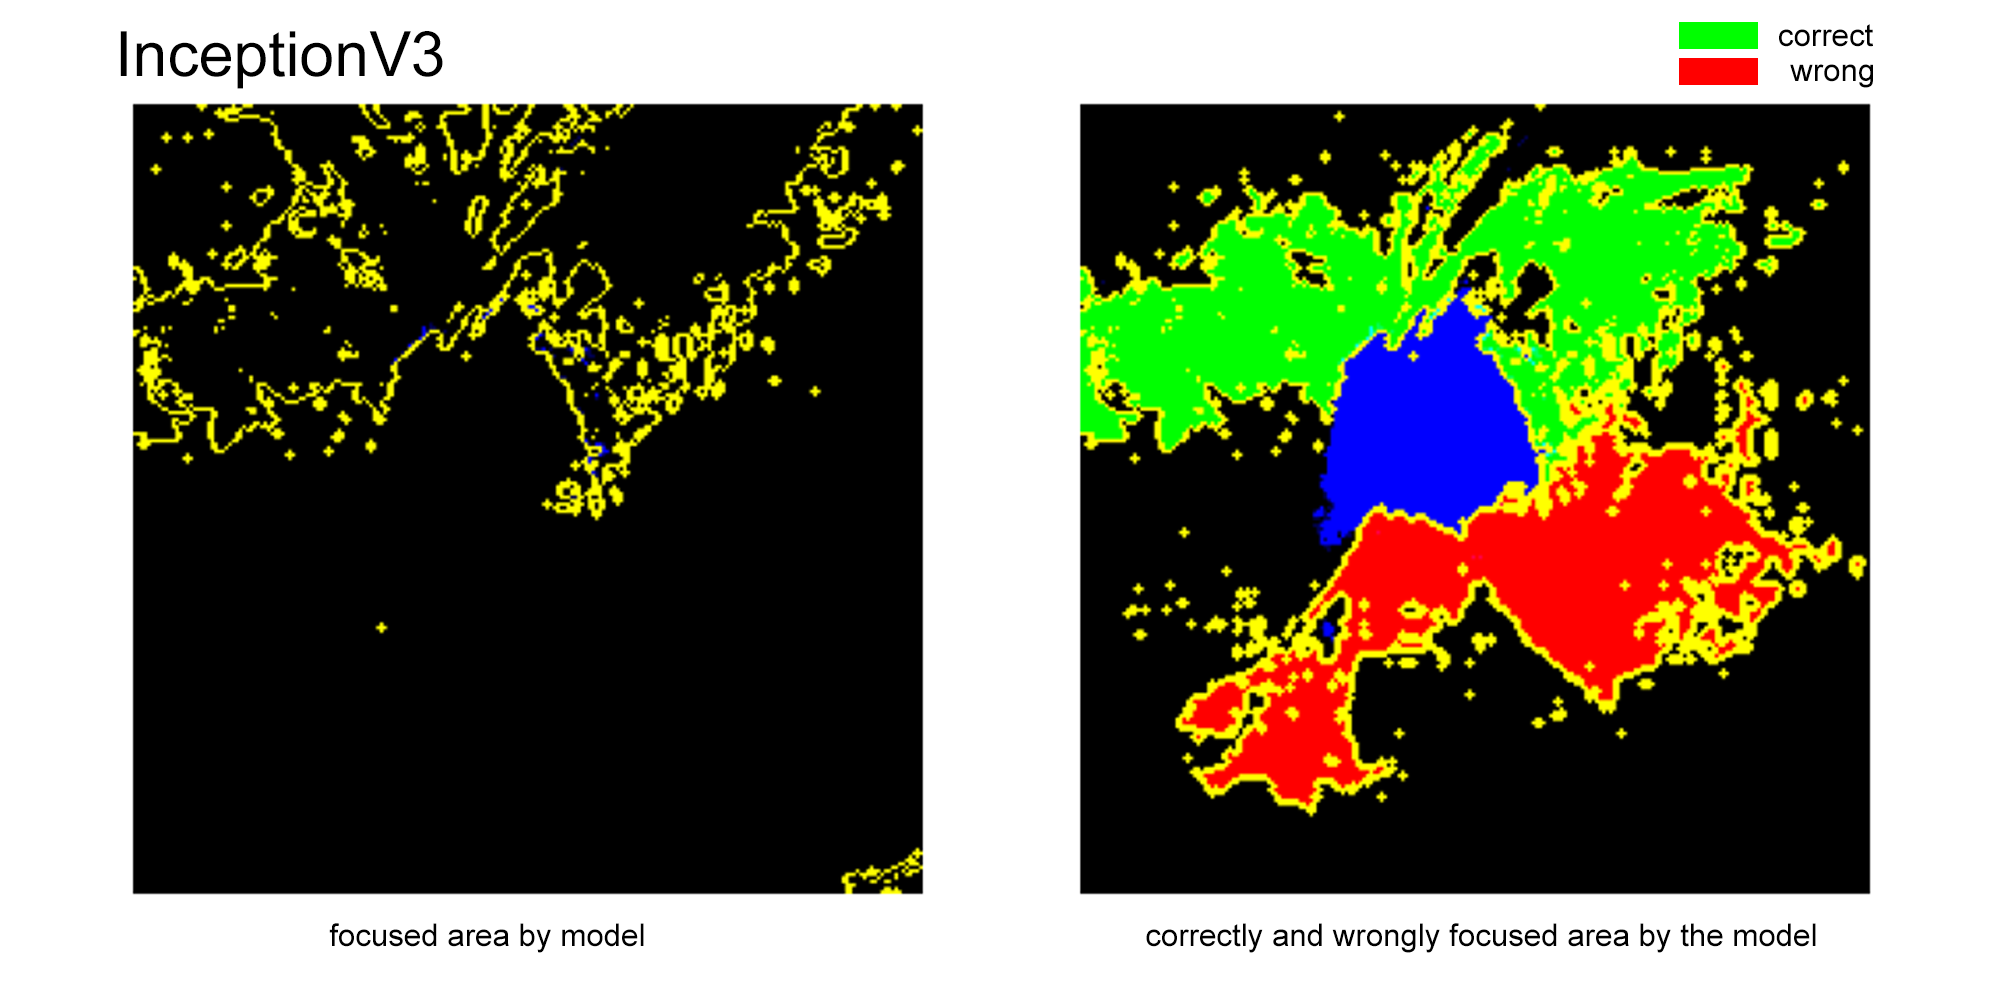
\includegraphics[scale=0.24]{fig-45.png}
\caption{Lime Explanation for InceptionV3}
\label{fig:x Lime Explanation for InceptionV3}
\end{figure}

\begin{figure}[hbt!]
\centering
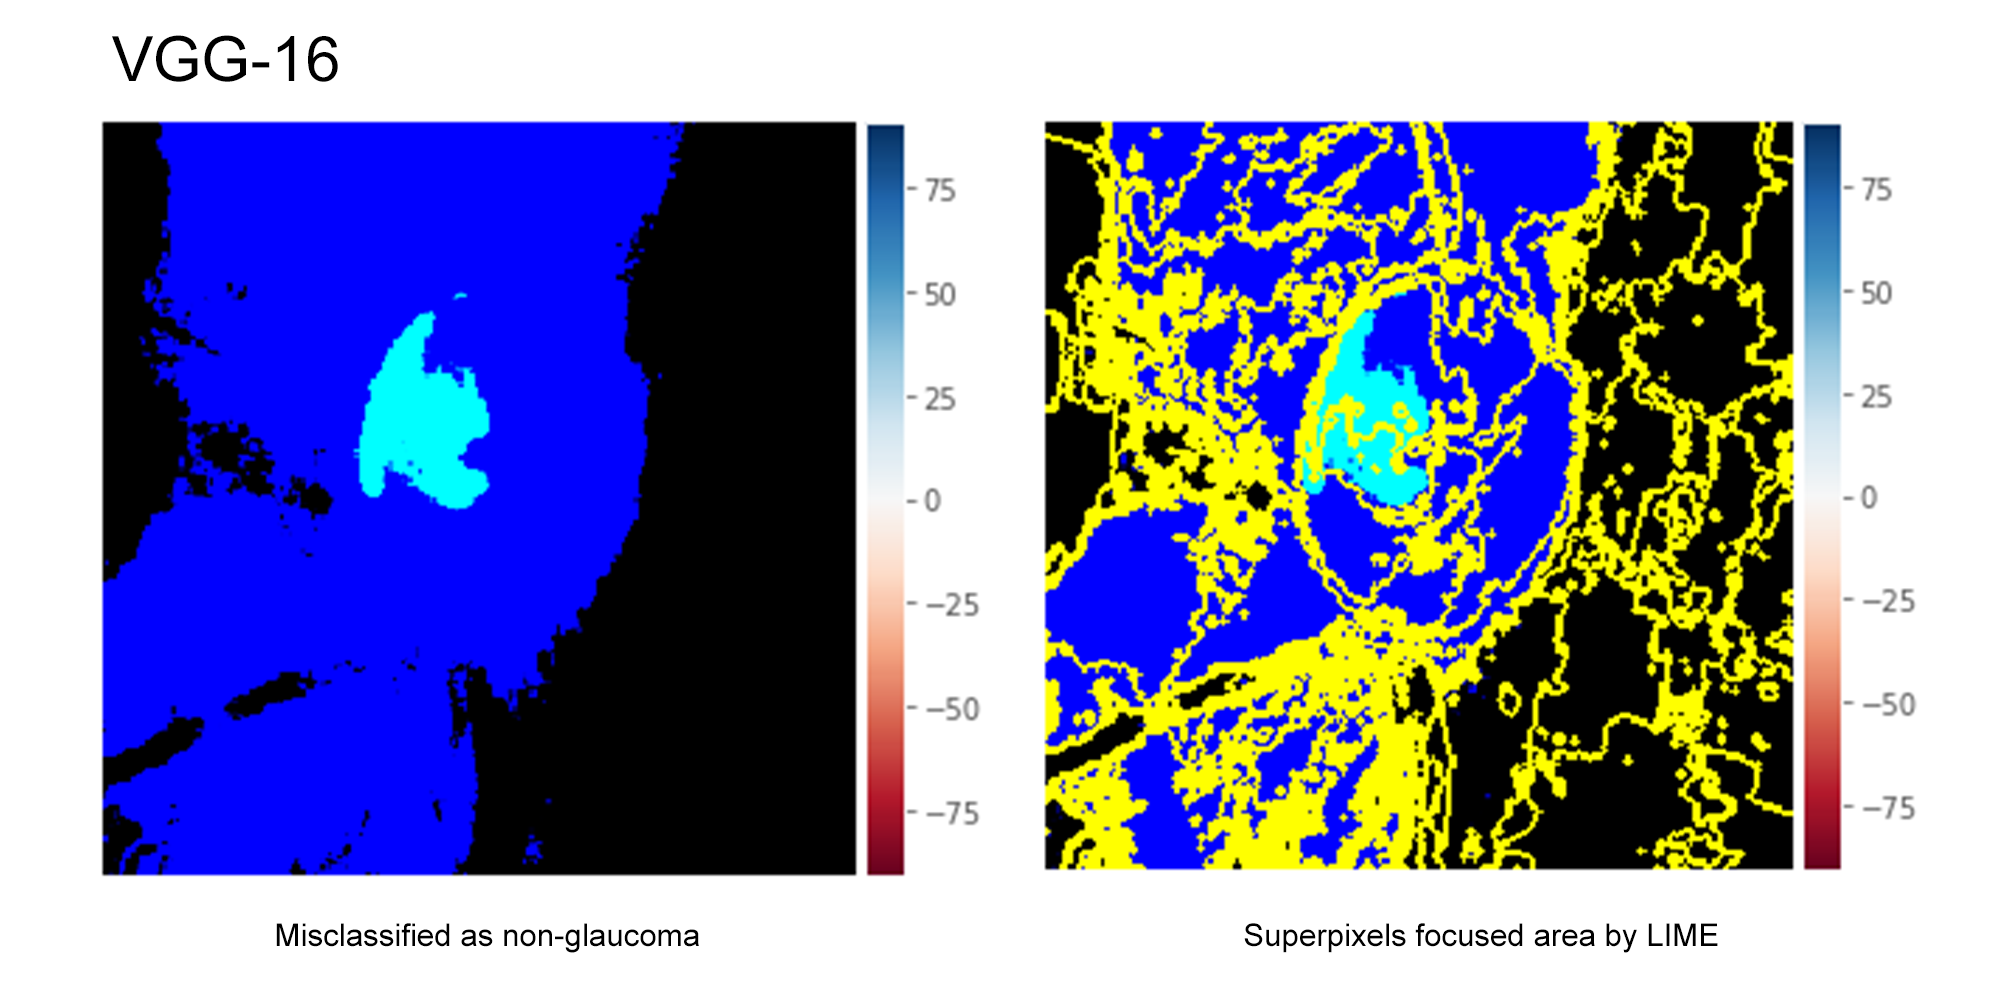
\includegraphics[scale=0.24]{fig-46.png}
\caption{Misclassified image with preprocessing and Superpixels focused area by Lime in VGG-16}
\label{fig:x Misclassified image with preprocessing and Superpixels focused area by Lime in VGG-16}
\end{figure}

\begin{figure}[hbt!]
\centering
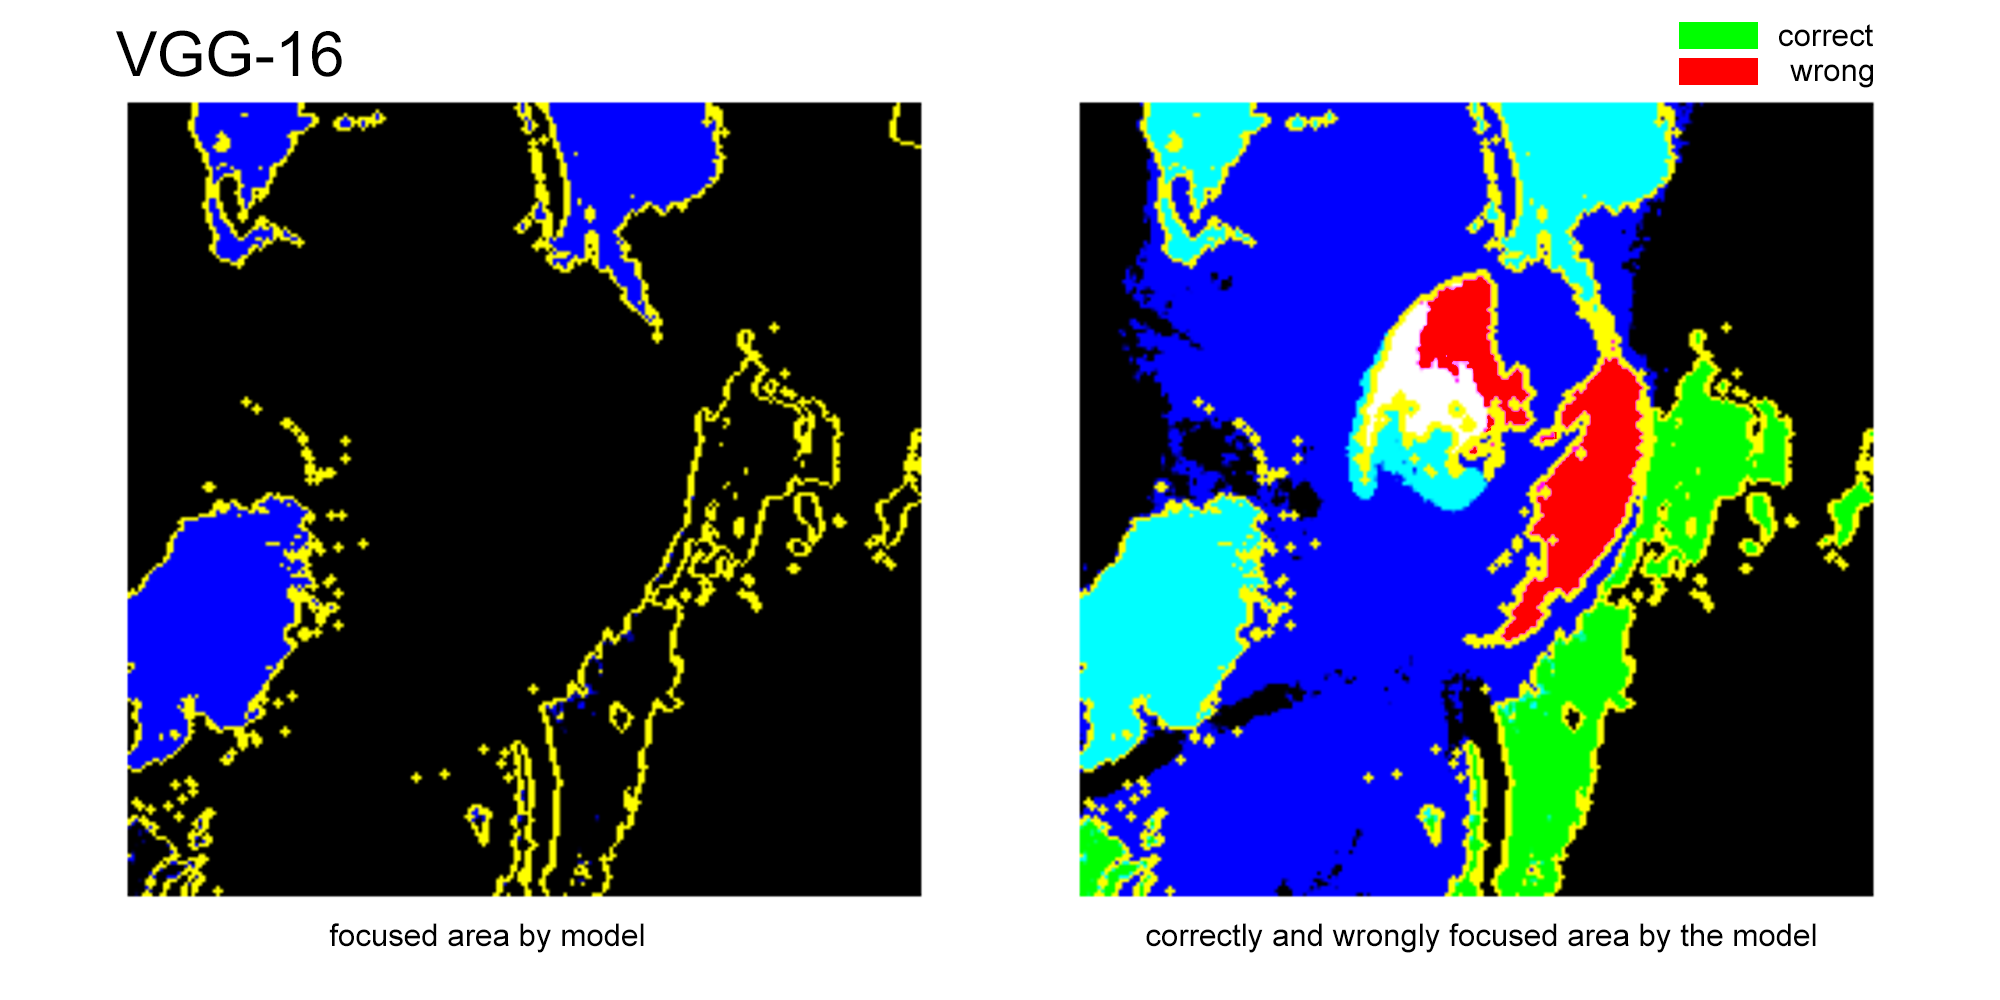
\includegraphics[scale=0.24]{fig-47.png}
\caption{Lime Explanation for VGG-16}
\label{fig:x Lime Explanation for VGG-16}
\end{figure}

\begin{figure}[hbt!]
\centering
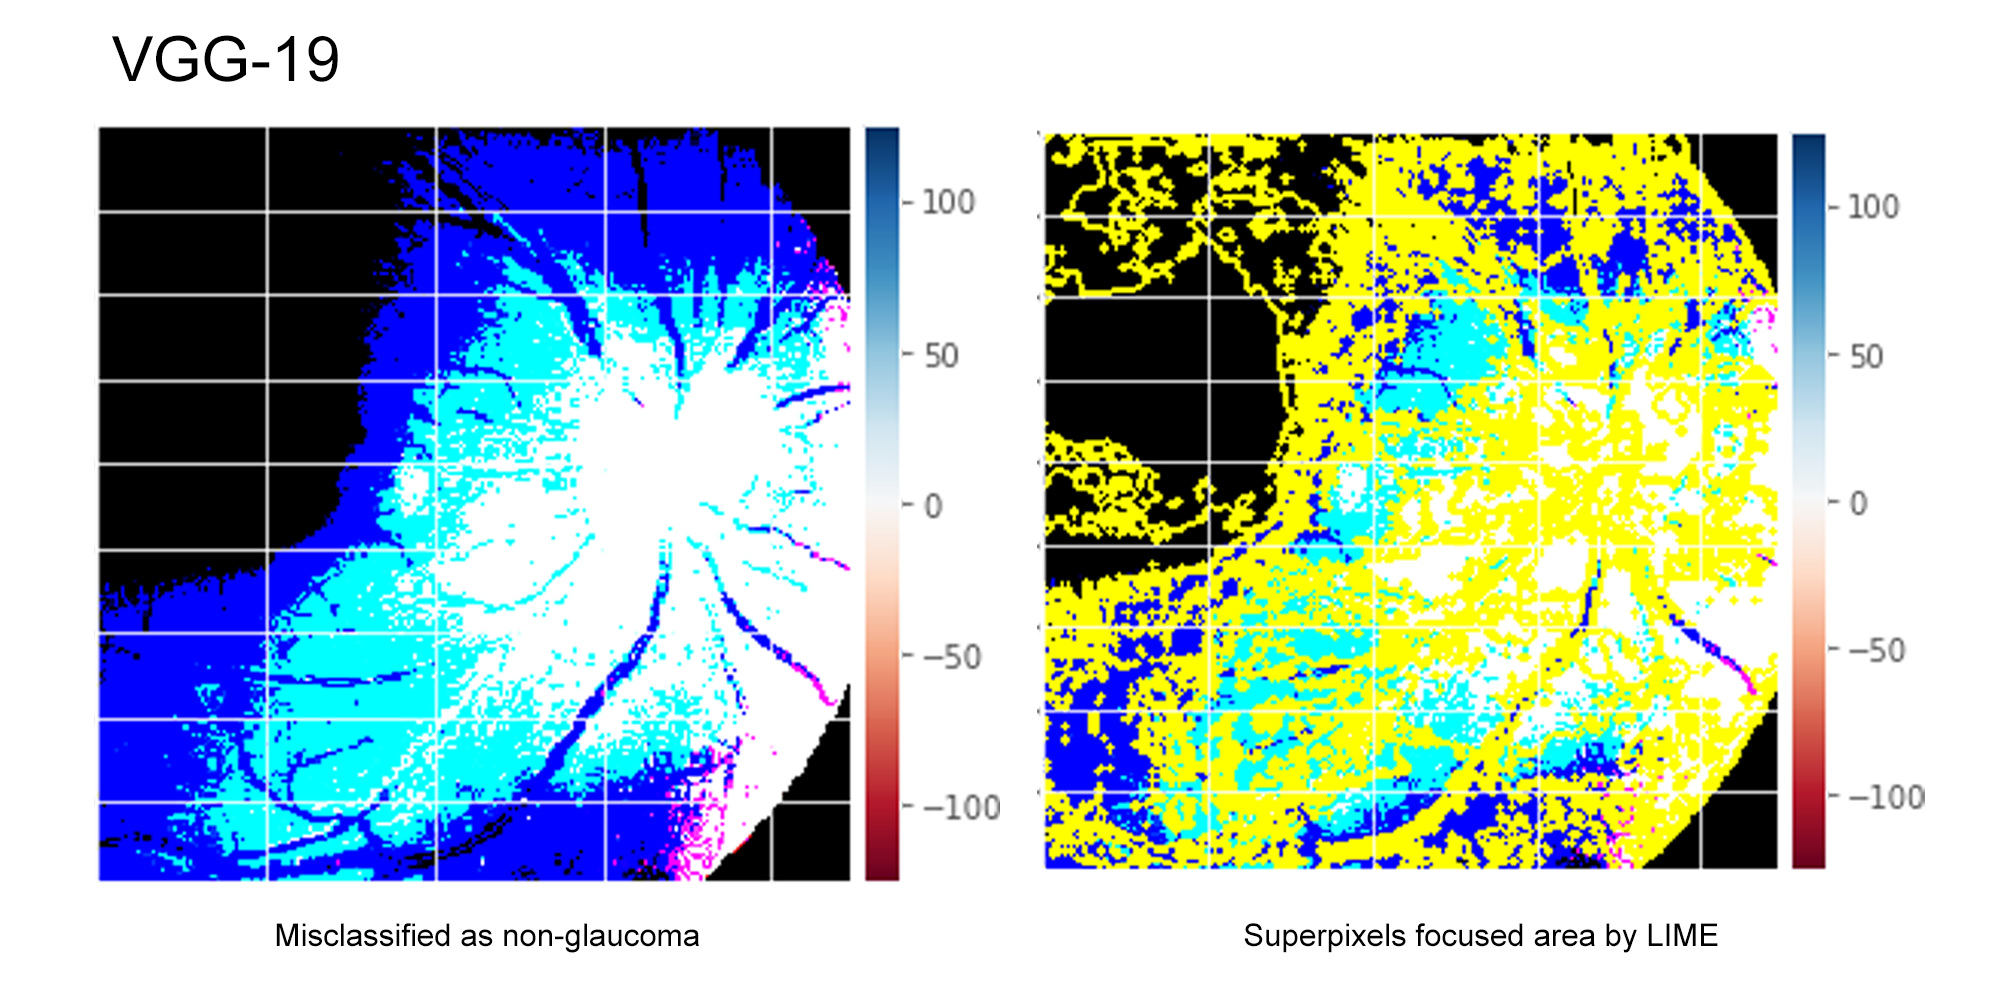
\includegraphics[scale=0.24]{fig-48.png}
\caption{Misclassified image with preprocessing and Superpixels focused area by Lime in VGG-19}
\label{fig:x Misclassified image with preprocessing and Superpixels focused area by Lime in VGG-19}
\end{figure}

\begin{figure}[hbt!]
\centering
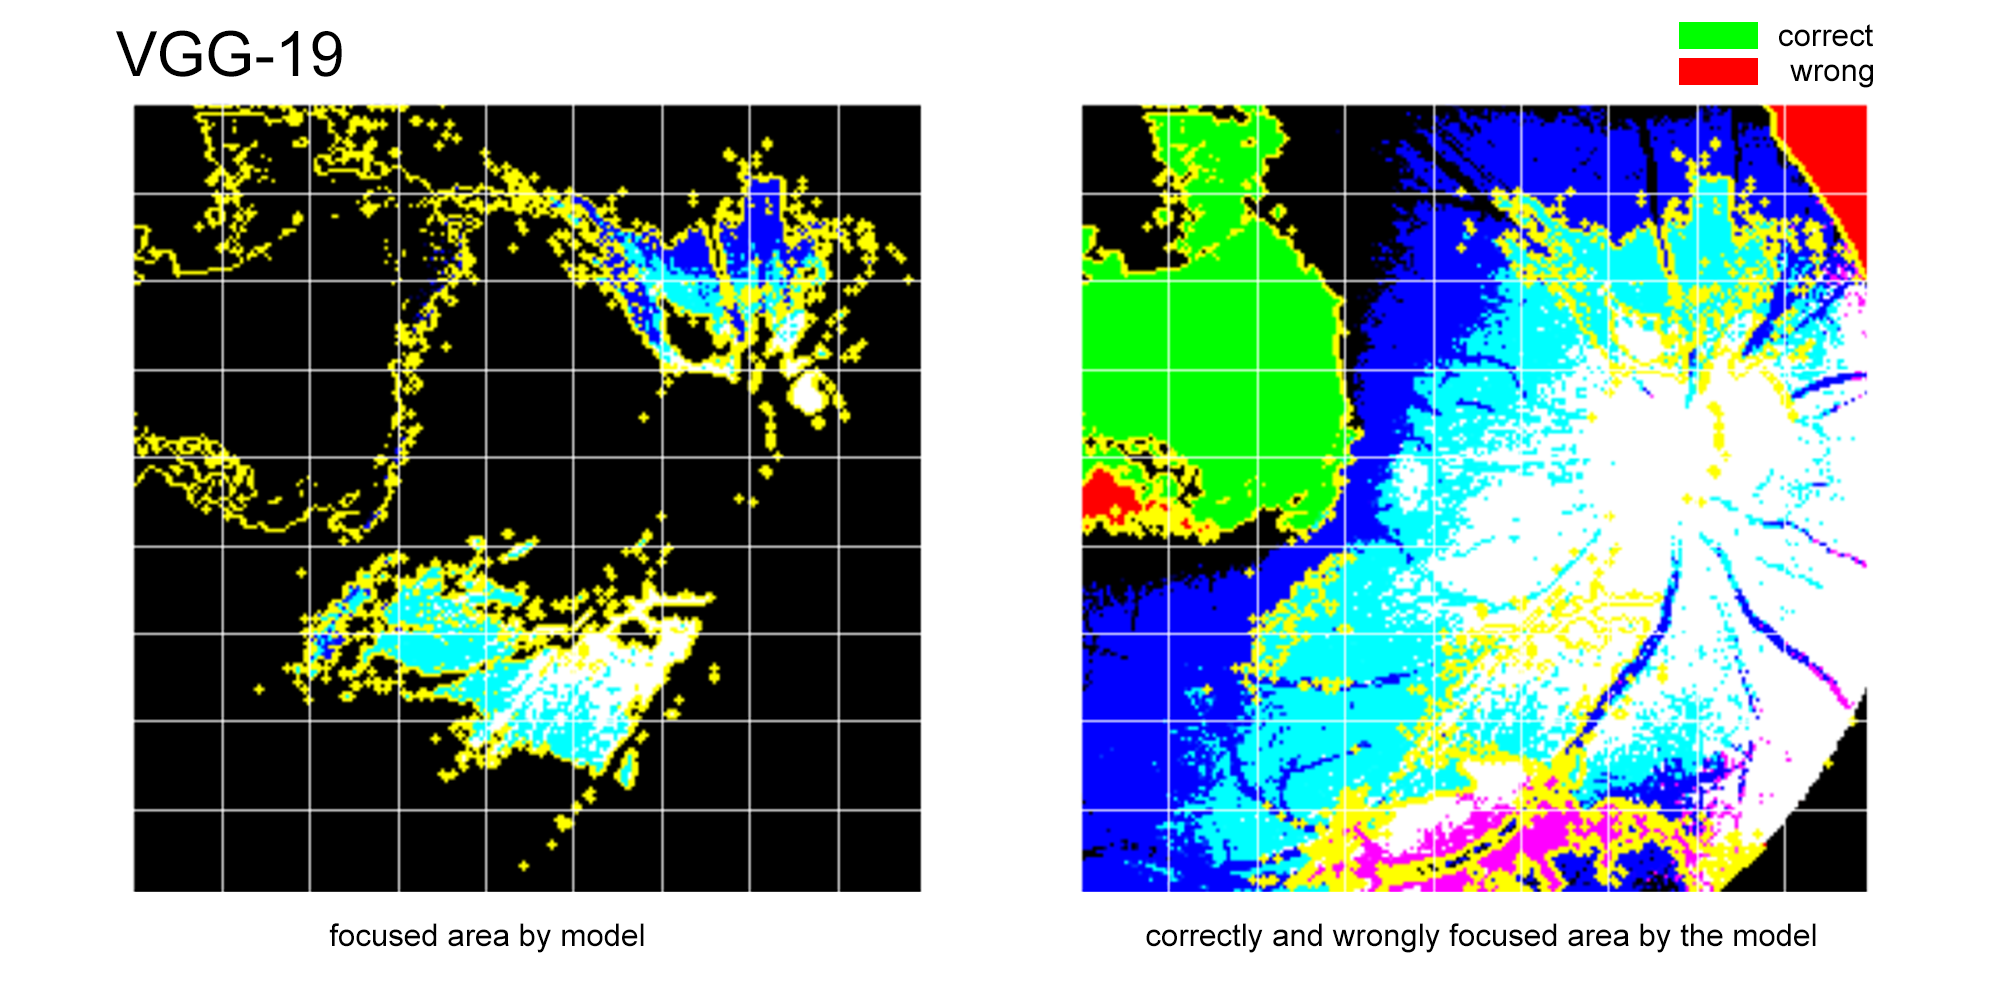
\includegraphics[scale=0.24]{fig-49.png}
\caption{Lime Explanation for VGG-19}
\label{fig:x Lime Explanation for VGG-19}
\end{figure}

\begin{figure}[hbt!]
\centering
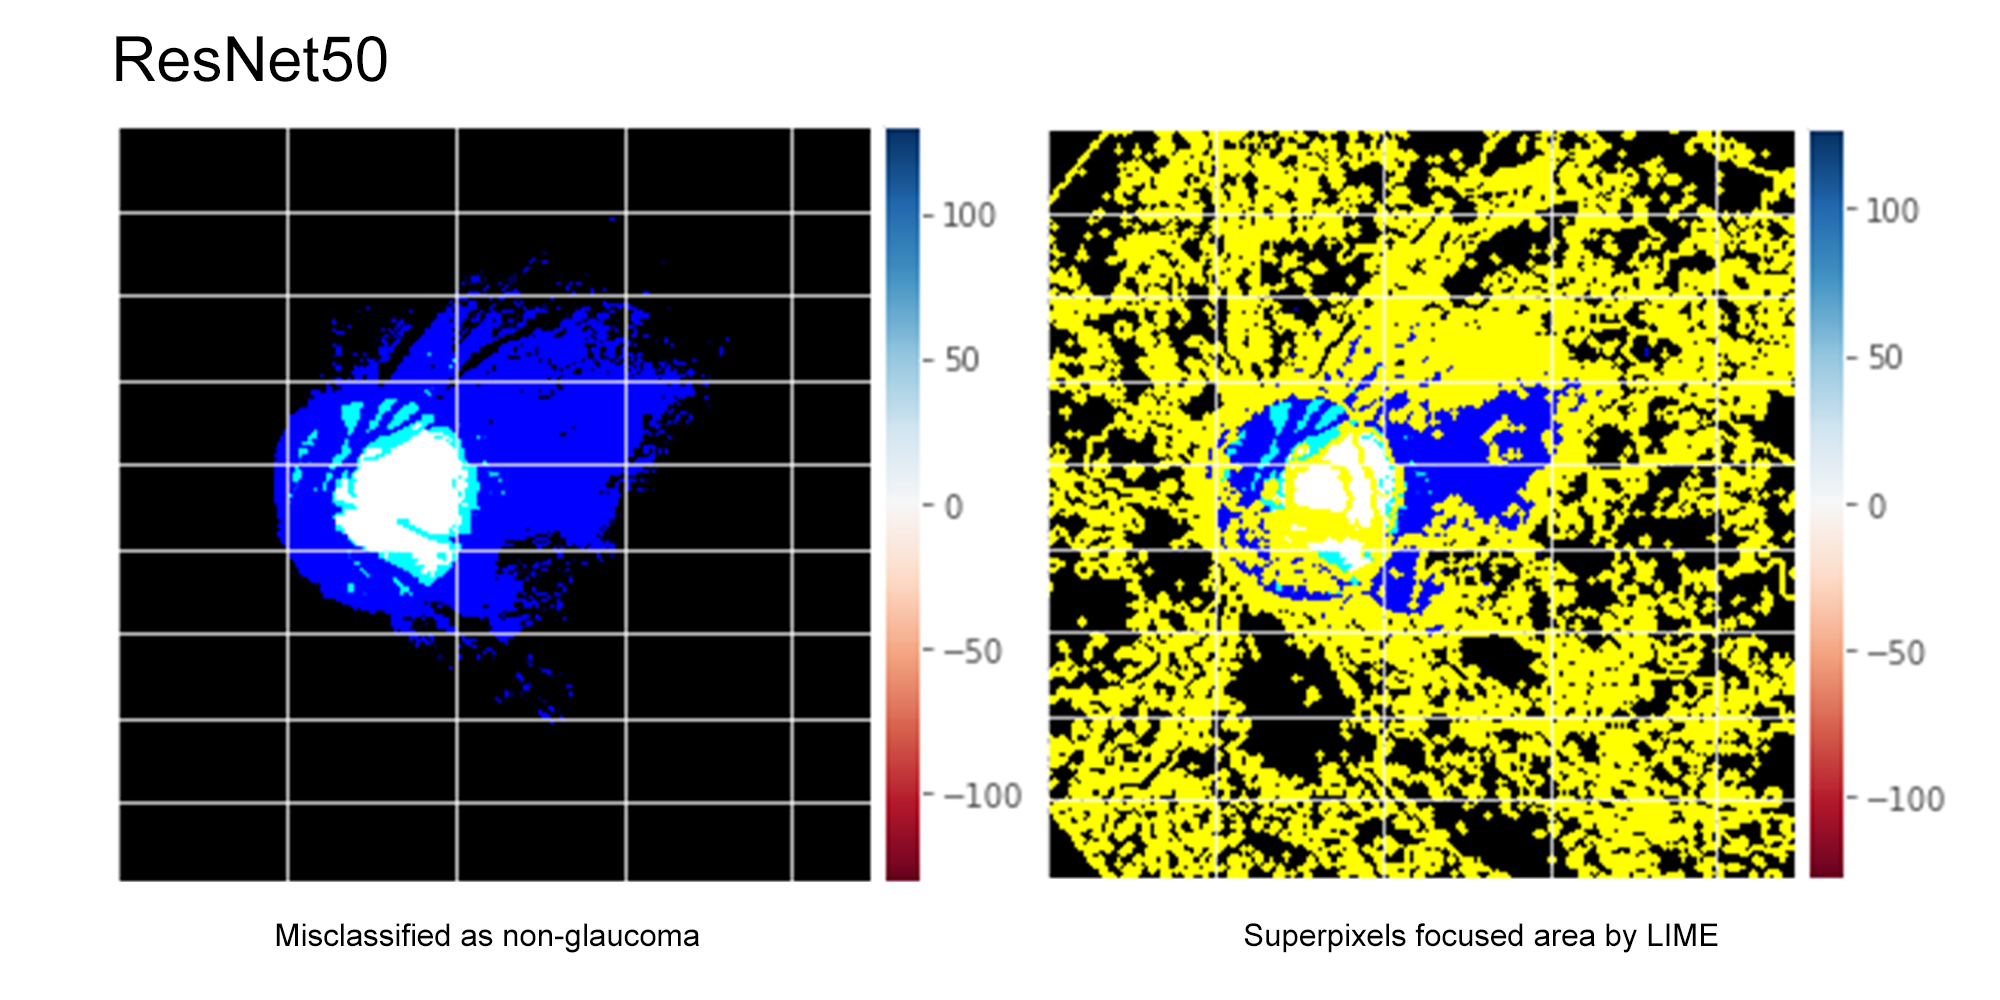
\includegraphics[scale=0.24]{fig-50.png}
\caption{Misclassified image with preprocessing and Superpixels focused area by Lime in ResNet50}
\label{fig:x Misclassified image with preprocessing and Superpixels focused area by Lime in ResNet50}
\end{figure}

\begin{figure}[hbt!]
\centering
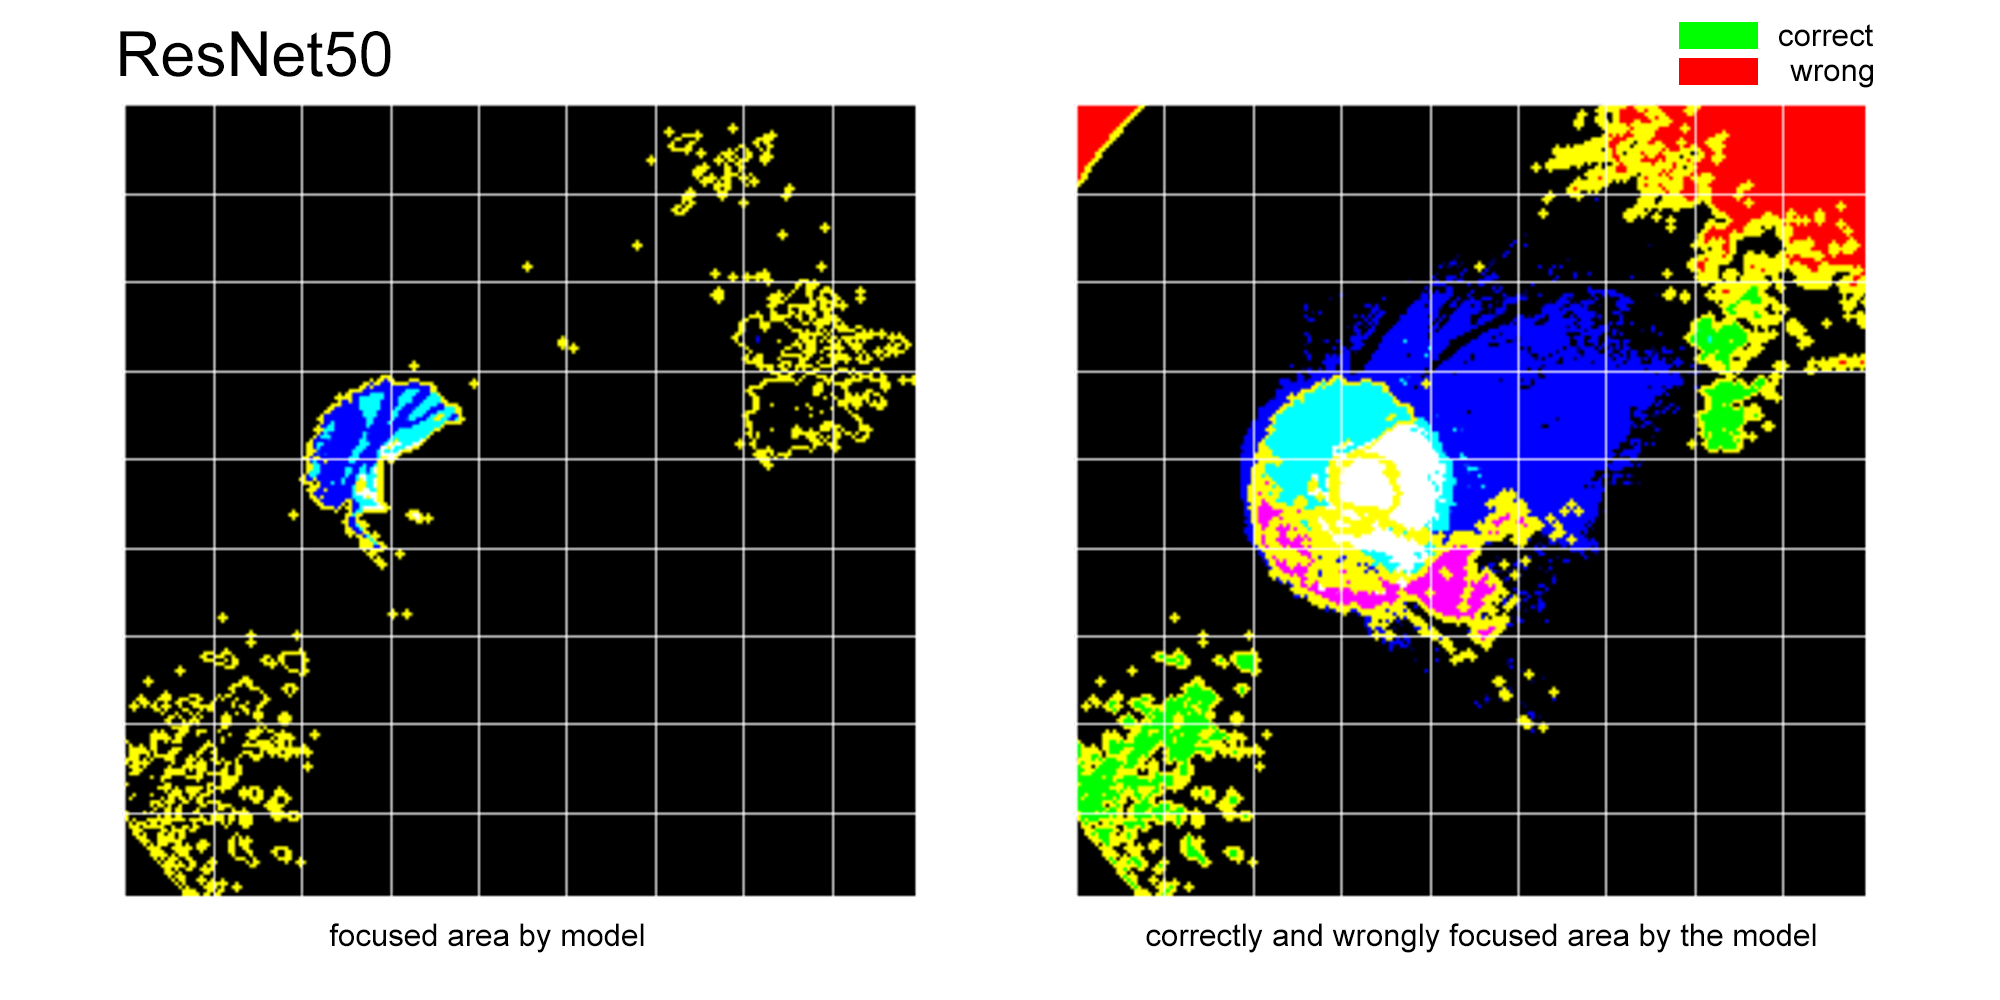
\includegraphics[scale=0.24]{fig-51.png}
\caption{Lime Explanation for ResNet50}
\label{fig:x Lime Explanation for ResNet50}
\end{figure}

 \noindent \textbf{In figure 31} we can see the the single predicted raw fundus image -

\begin{figure}[hbt!]
\centering
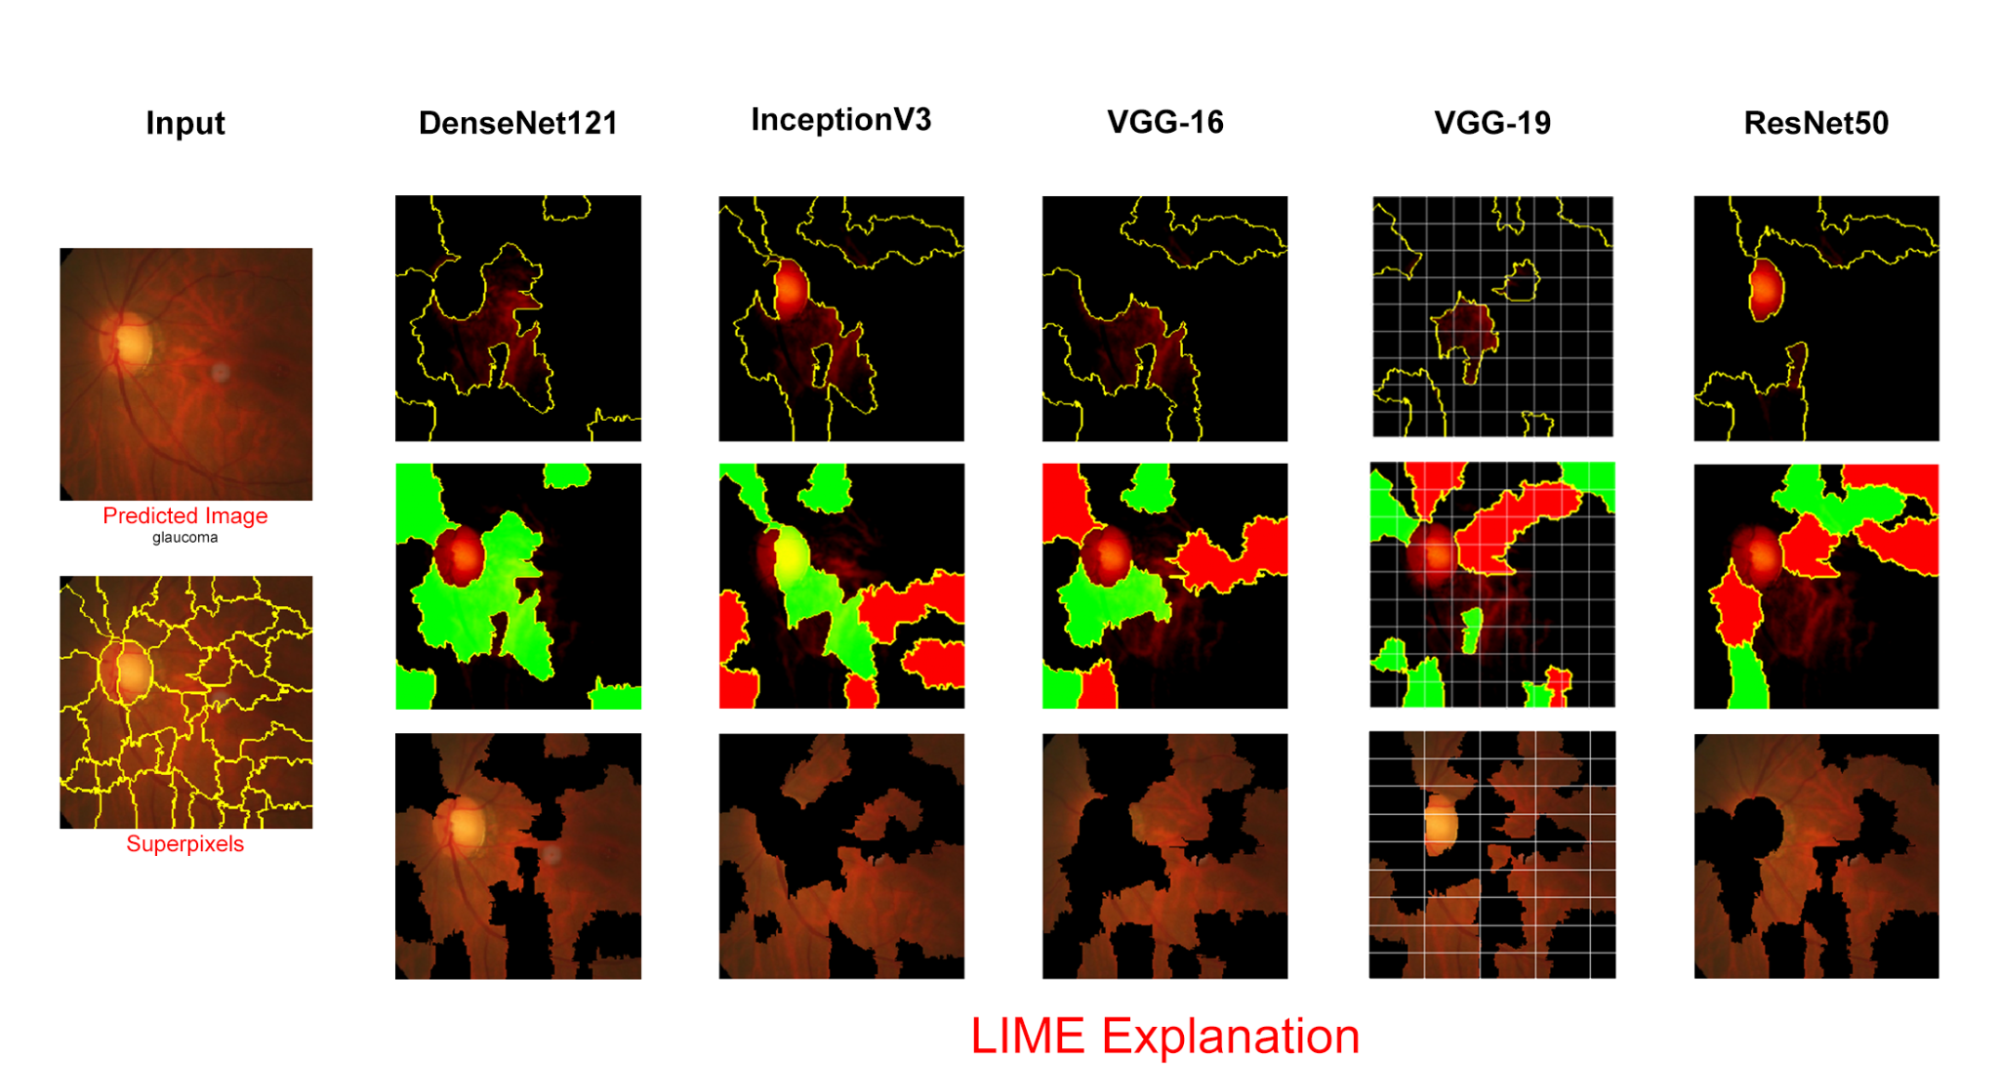
\includegraphics[scale=0.12]{fig-52.png}
\caption{Lime Explanation for all models single image predictions}
\label{fig:x Lime Explanation for all models single image predictions}
\end{figure}

\newpage
\section{Conclusion}
\subsection{Challanges}

The goal of our research has been successfully achieved. But to achieve what we desired we had to go through some difficulties or obstacles, which we had to tackle. At first in our model overfitting issues occurred VGG-16 and InceptionV3 got overfitted as the train loss curve goes under the value loss curve or on the other hand train accuracy is much higher than the validation accuracy. Also the DenseNet121 is underfitted as the training loss is over the validation loss. Then we increased our datasample to overcome overfitting. Moreover, the pandemic situation made it more difficult for us as we had to work from home which caused no access to university resources,  one of which was a high-performance computer with GPU, so we had to rely on Jupyter Notebook at the first time, but then we managed to work with GPU. As a result, training took a long time to get the results and we had frequent network problems as well. 

\subsection{Limitations}

Leaving aside what we have successfully done, there remain a few roadblocks that must be overcome. The lack of processing resources, such as the GPU's limits, is a key impediment to this study. Due to the poor GPU, the training phase took substantially longer because the dataset we utilized was fairly large. We also had difficulties with categorization and prediction since we trained on lesser datasets. We were able to tackle this problem by supplementing an existing dataset with new data. We could have avoided this scenario if we had used a more powerful GPU. We also manually mapped, which may have been done automatically. Afterwards, our future goal is to improve this research to make the glaucoma detection more easier and faster than it exists now. 

\subsection{Future Works}

Afterwards, our future goal is to improve this research to make the glaucoma detection more easier and faster than it exists now. Till now we have detected Glaucoma and Non-Glaucoma at a satisfactory accuracy rate using multiple models but in near future we are planning to develop a web application which will help people to identify Glaucoma by just uploading the images. Moreover, we are planning to work on more datasets with improved accuracy. 

\subsection{Conclusion}

In this research, to attain the ultimate objective of our study in Glaucoma Diagnosis, the Black Box model was defined using Explainable Artificial Intelligence (XAI). Notably, glaucoma can take away the vision of a patient which is why it’s more important to work for a better solution for early stage detection of glaucoma disease. To serve our purpose, we can see that in InceptionV3 we got 86.4\% accuracy, in DenseNet121 we got 86.8\% accuracy, in ResNet50 we got 94.7\% accuracy, in VGG-19 we got 93.3\% accuracy and lastly in VGG-16 we got 88.6\% accuracy.  RestNet50 got the highest score among the other models with a validation accuracy of 94.7\%.  Afterwards we compared all models' accuracy and loss graph together, where we can see that VGG-19 and ResNet50 were the Good-Fit than the other models. To sum up, we can say this research has achieved the goal to bring more accuracy, reliability and commitment to improve more in early stage glaucoma detection.

\subsection{Acknowledgement }

Firstly, all praise to the almighty Allah for whom our thesis has been completed without any major interruption. Secondly, to our supervisor MD Tanzim Reza sir for his kind support and advice in our work. Sir supervised us whenever we needed help. And finally to our parents without their thorough support it may not be possible. With their kind support and prayer we are now on the verge of our graduation.

\begin{thebibliography}{00}
\bibitem{b1} GSalam, A. A., Khalil, T., Akram, M. U., Jameel, A., Basit, I. (2016). Automated detection of glaucoma using structural and non structural features. SpringerPlus, 5(1).
\bibitem{b2} Ran, A., Cheung, C. Y. (2021). Deep Learning-Based Optical Coherence Tomography and Optical Coherence Tomography Angiography Image Analysis: An Updated Summary. Asia-Pacific Journal of Ophthalmology, 10(3), 253–260.
\bibitem{b3} Aleci, C. (2020). Detection of Visual Field Loss Progression in Glaucoma: An Overview and Food for Thought. Ophthalmology Research: An International Journal, 16–24.
\bibitem{b4} Diabetic Retinopathy — National Eye Institute. (2021, July 30). National Eye Institute.
\bibitem{b5} Types of Glaucoma.(2020, June 2). Glaucoma Research Foundation. 
\bibitem{b6} aba, T., Khan, M. W., Yasmin, M., Sharif, M. (2017). CDR based glaucoma detection using fundus images: a review. International Journal of Applied Pattern Recognition, 4(3), 261.
\bibitem{b7} Thakoor, K. A., Li, X., Tsamis, E., Sajda, P., Hood, D. C. (2019). Enhancing the Accuracy of Glaucoma Detection from OCT Probability Maps using Convolutional Neural Networks. 2019 41st Annual International Conference of the IEEE Engineering in Medicine and Biology Society (EMBC).
\bibitem{b8} Lim, T. C., Chattopadhyay, S., Acharya, U. R. (2012). A survey and comparative study on the instruments for glaucoma detection. Medical Engineering Physics, 34(2), 129–139.
\bibitem{b9} Abbas, Q. (2017). Glaucoma-Deep: Detection of Glaucoma Eye Disease on Retinal Fundus Images using Deep Learning. International Journal of Advanced Computer Science and Applications, 8(6).
\bibitem{b10} Dervisevic, E., Pavljasevic, S., Dervisevic, A., Kasumovic, A. (2016). Challenges In Early Glaucoma Detection. Medical Archives, 70(3), 203. 
\bibitem{b11} Mayro, E.L., Wang, M., Elze, T. et al. The impact of artificial intelligence in the diagnosis and management of glaucoma. Eye 34, 1–11 (2020). 
\bibitem{b12} Greco, A., Rizzo, M. I., De Virgilio, A., Gallo, A., Fusconi, M., de Vincentiis, M. (2016). Emerging concepts in Glaucoma and review of the literature. The American Journal of Medicine (2016).
\bibitem{b13} Pascolini, D., Mariotti, S. P. (2012). Global estimates of visual impairment: 2010. British Journal of Ophthalmology, 96(5), 614-618. 
\bibitem{b14} Murphy, A. M., Moore, C. M. M. (2020). Fully connected neural network.
\bibitem{b15} Khan, S. M. K. (2021, January 3). Papers with Code - LAG Dataset. The Lancet.
\bibitem{b16} How to fine-tune your artificial intelligence algorithms. (2020, January 13). Allerin.
\bibitem{b17} Da˘glarli, E. (2020). Explainable Artificial Intelligence (XAI) Approaches and Deep Meta-Learning Models. Advances and Applications in Deep Learning, 79. 
\bibitem{b18} Vejjanugraha, P., Kongprawechnon, W., Kondo, T., Tungpimolrut, K., Kotani, K. (2017). An automatic screening method for primary open-angle glaucoma assessment using binary and multi-class support vector machines. ScienceAsia, 43(4), 229.

\end{thebibliography}

\end{document}
